

Following the iterative development process outlined in the previous section, the final design of the visualization framework presents an interface that integrates spatial and symbolic representations of $\text{LORE}_{sa}$ explanations and that could easily be repurposed to accommodate other explainability methods. The system workflow is separated into two primary components: an \textbf{interactive configuration interface} that enables comprehensive control over the explanation generation process, and a \textbf{coordinated visualization system} that presents the resulting explanations through two interconnected views.

The final implementation represents the end of our design evolution, incorporating lessons learned from each development phase to create a comprehensive interactive explanation system. The interface employs a \textbf{progressive disclosure workflow} \cite{readingsInformationVi} that guides users through sequential configuration steps while maintaining access to previously configured options.

\section{Configuration Interface Architecture}

The configuration interface implements, a \textbf{vertically-stacked progressive workflow} that structures the explanation generation process into, in its demo form, seven sequential but revisable stages: dataset selection, classifier selection, classifier parameter configuration, instance specification, explanation parameter settings, dimensionality reduction techniques parameter settings, and visualization selection. This sequential presentation reduces cognitive load by presenting configuration options in logical order while allowing users to revisit previous steps.

\textbf{Workflow Progression Design}: Each configuration stage employs \textbf{scroll-based navigation} with automatic scrolling to newly revealed sections, providing clear visual feedback about workflow progression. Completed sections remain visible above the current configuration step, enabling users to verify previous selections and modify settings as needed. The interface implements \textbf{state preservation} across section transitions, maintaining user selections even when navigating backward through the workflow.

\subsection{Dataset Selection Interface}

\begin{figure}[htbp]
    \centering
    \begin{subfigure}[c]{\textwidth}
        \centering
        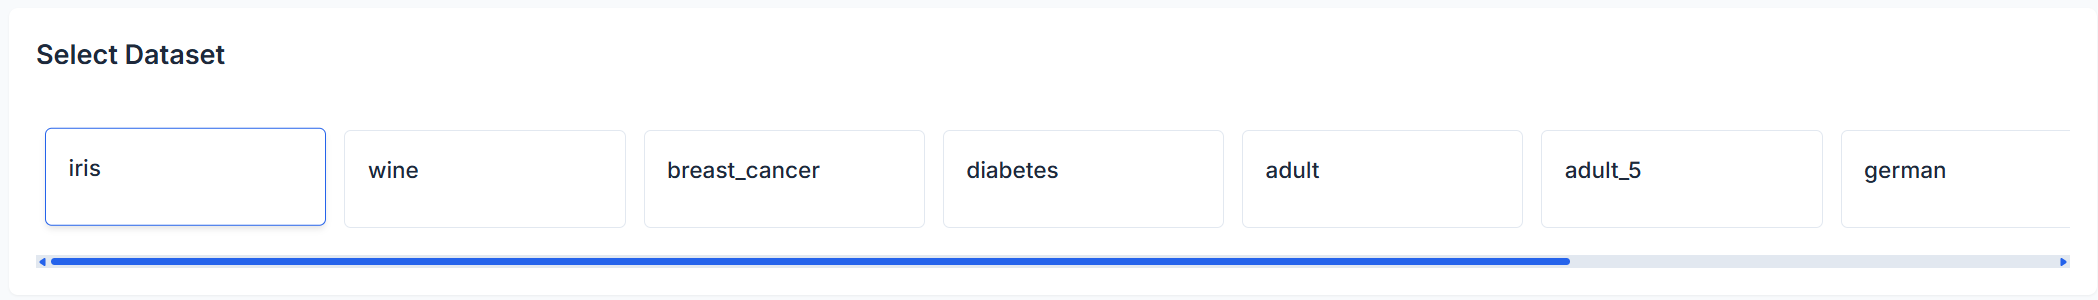
\includegraphics[width=\textwidth]{images/datasetSelectionComponentBefore.png}
        \caption{Before dataset selection with hover interaction.}
    \end{subfigure}
    \vfill
    \begin{subfigure}[c]{\textwidth}
        \centering
        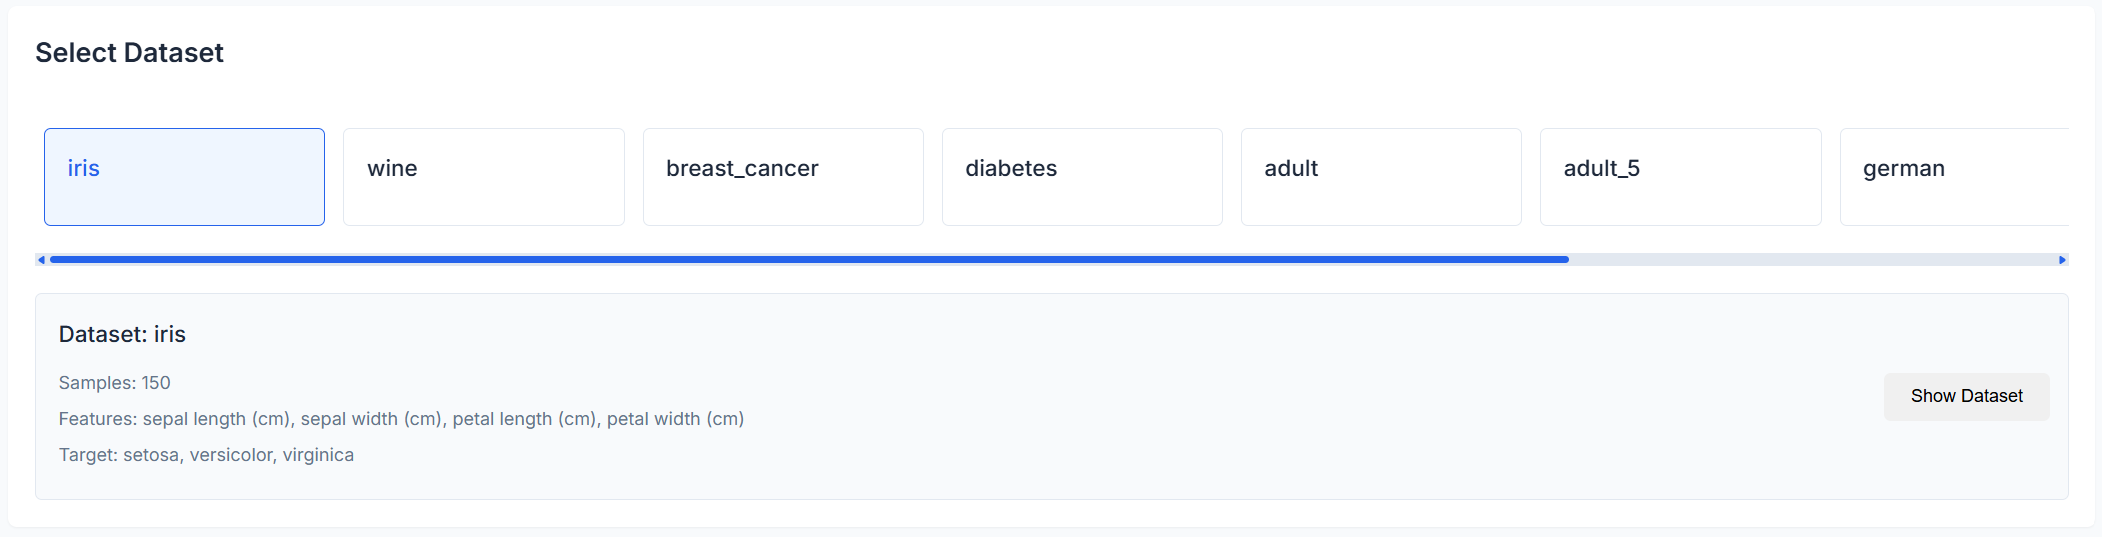
\includegraphics[width=\textwidth]{images/datasetSelectionComponentAfter.png}
        \caption{After dataset selection.}
    \end{subfigure}

    \caption{Dataset selection component.}
    \label{fig:datasetSelectionInterface}
\end{figure}

The dataset selection component, shown in Figure \ref{fig:datasetSelectionInterface} provides the workflow entry point through a \textbf{grid-based card layout} that presents available datasets with contextual information. Each dataset is represented by a distinct card containing the dataset name, basic descriptive information, and selection affordances.
%
% \textbf{Visual Card Design}: 
Dataset cards employ \textbf{hover-based visual feedback} with subtle elevation changes and border highlighting to indicate interactive affordances. The selected dataset receives persistent highlighting through distinct border coloring and background shading, providing clear visual confirmation of the current selection state.
% 
% \textbf{Information Disclosure}: 
Upon dataset selection, an \textbf{information panel} appears, revealing dataset metadata including size, feature and target names. A dedicated "Show Dataset" button triggers a \textbf{slide-in panel} from the right side of the interface that displays the complete dataset in tabular format, enabling users to inspect actual data values and understand dataset characteristics before proceeding with explanation generation.

The dataset display panel, shown in Figure \ref{fig:showDatasetPanel} implements \textbf{responsive table styling} with horizontal scrolling for wide datasets and header rows. A close button in the top right enables dismissal of the dataset panel without disrupting the main workflow.

\begin{figure}[htbp]
  \centering
  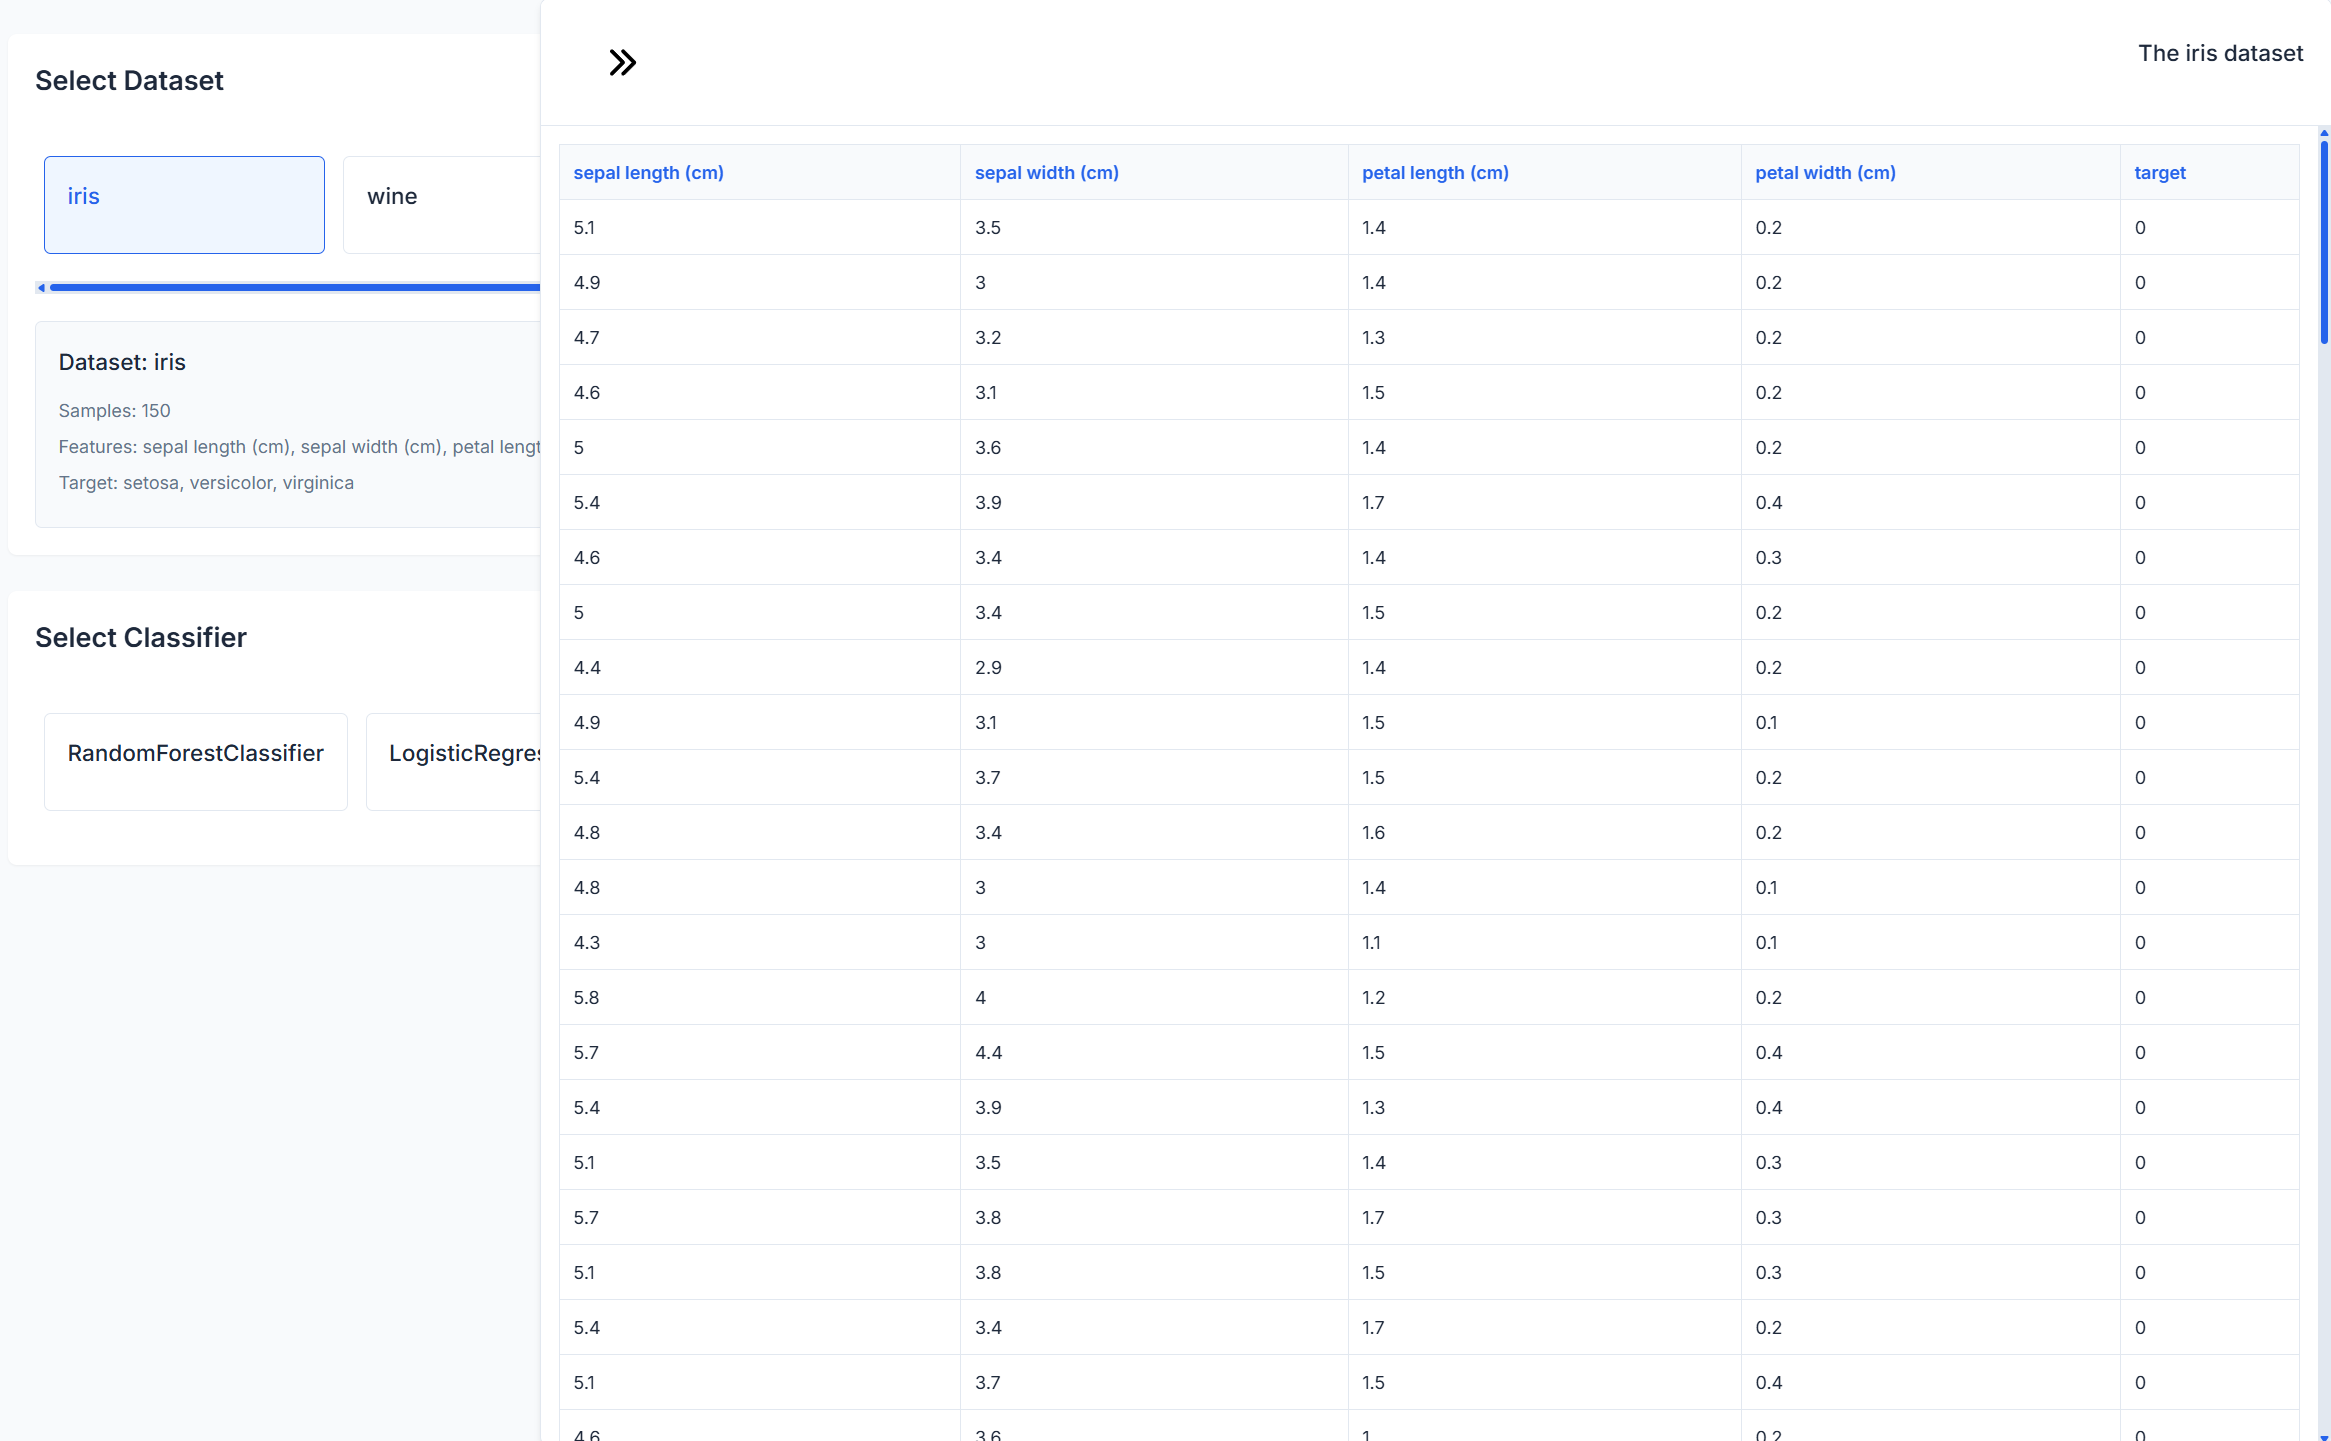
\includegraphics[width=0.9\textwidth]{images/showdatasetpanel.png}
  \caption{Dataset show panel.}
  \label{fig:showDatasetPanel}
\end{figure}

\subsection{Classifier Selection Interface}

\begin{figure}[htbp]
    \centering
    \begin{subfigure}[c]{\textwidth}
        \centering
        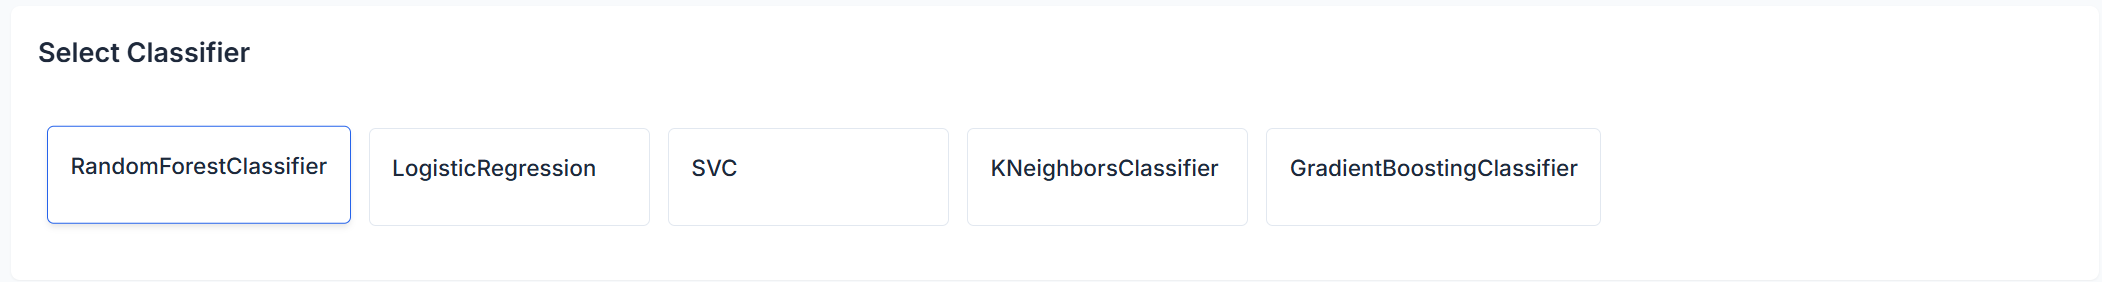
\includegraphics[width=\textwidth]{images/classifierSelectionComponentBefore.png}
        \caption{Before classifier selection with hover interaction.}
    \end{subfigure}
    \vfill
    \begin{subfigure}[c]{\textwidth}
        \centering
        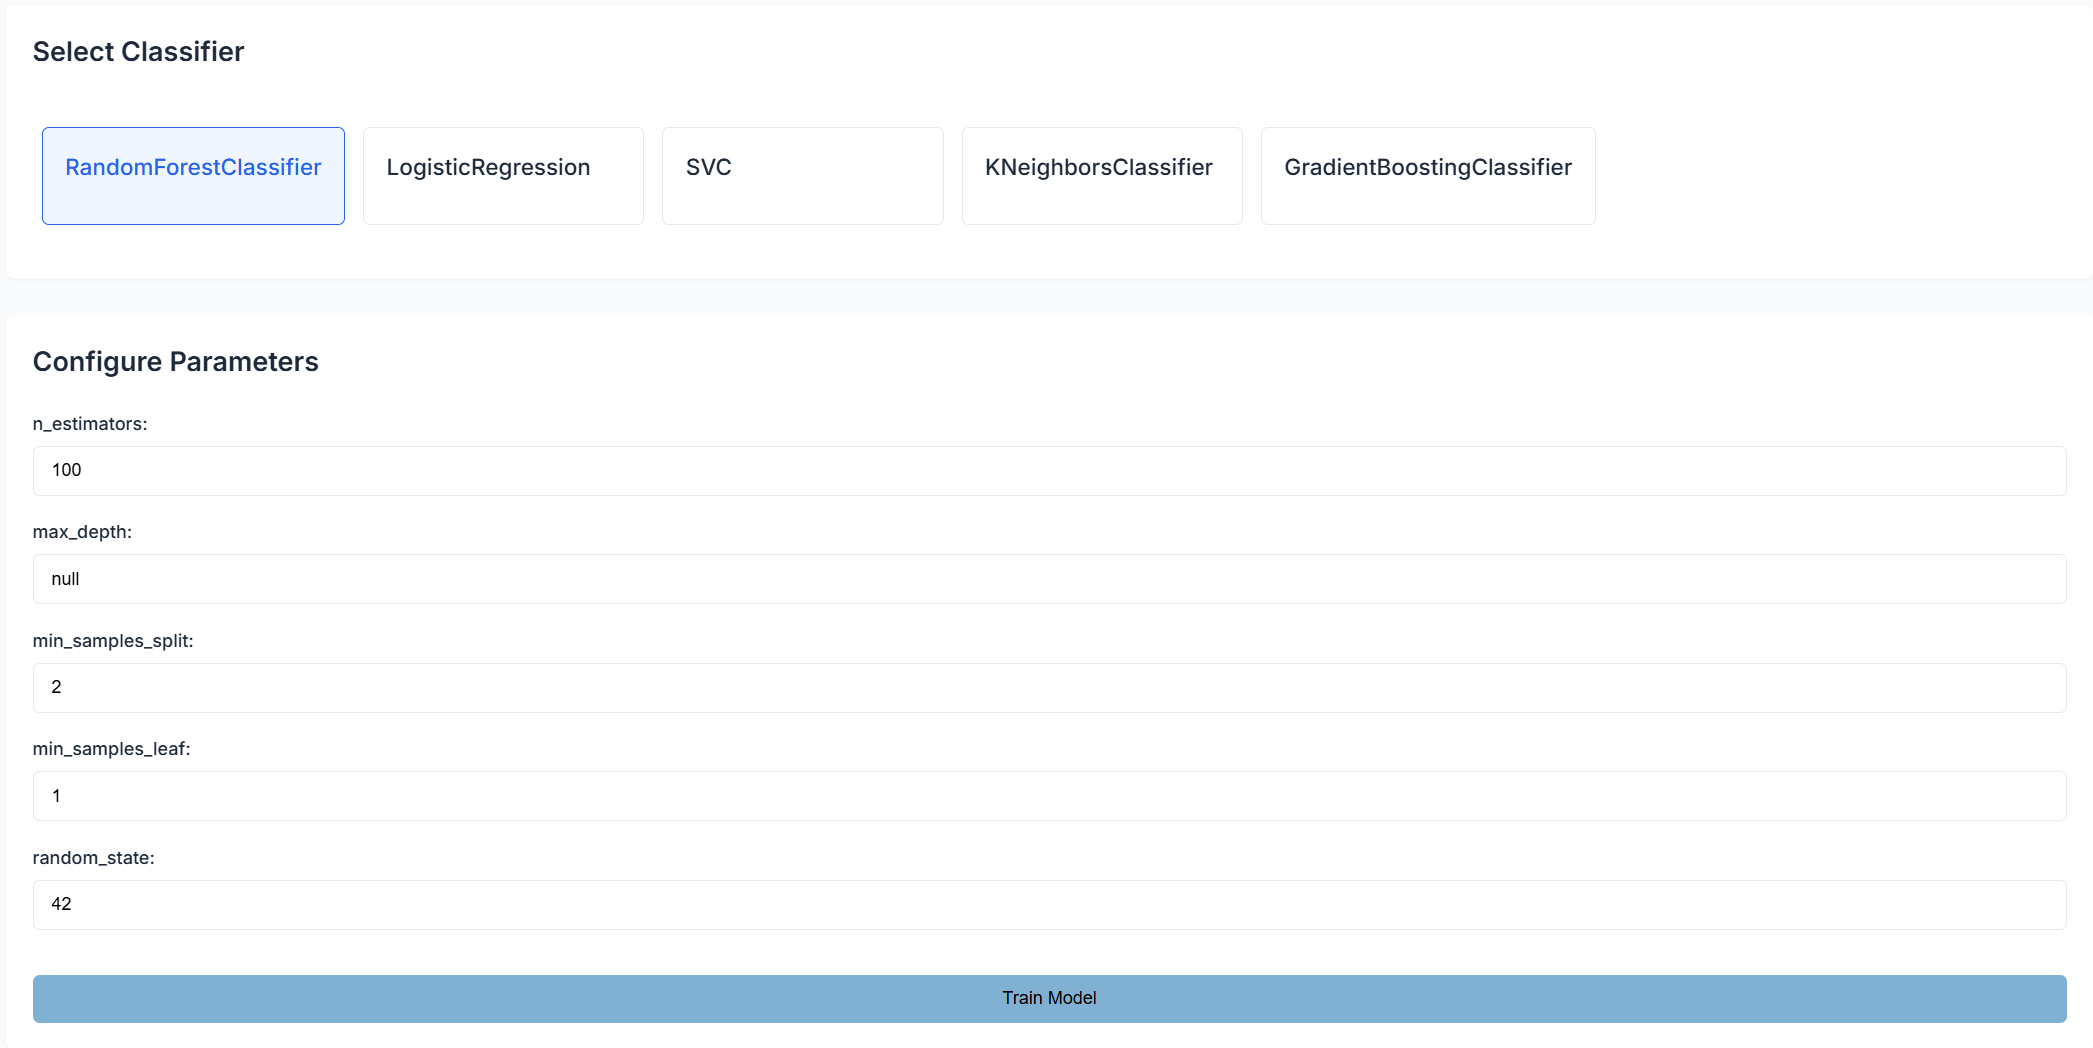
\includegraphics[width=\textwidth]{images/classifierSelectionComponentAfter.png}
        \caption{After classifier selection.}
    \end{subfigure}

    \caption{Classifier selection component.}
    \label{fig:classifierSelectionGrid}
\end{figure}

Following dataset selection, the interface reveals the \textbf{classifier selection grid}, shown in Figure \ref{fig:classifierSelectionGrid} that presents available classification algorithms. The grid layout maintains visual consistency with the dataset selection interface while adapting to the number of available classifiers.
% 
% \textbf{Classifier Cards}: 
Each classifier card displays the algorithm name and maintains the same interaction patterns as dataset cards. The interface supports common classification algorithms, including Random Forest, Support Vector Machines, Gradient Boost Classifier, and others, with the specific set of available classifiers dynamically populated from the backend system.
% 
% \textbf{Seamless Transition}: 
The classifier selection section appears immediately below the dataset information panel through smooth scrolling animation, maintaining visual continuity in the workflow progression. The system preserves dataset selection state, allowing users to modify classifier choice without requiring dataset reselection.

\subsection{Classifier Parameter Configuration Interface}

The parameter configuration section dynamically generates appropriate input controls based on the selected classifier's possible hyperparameters. This \textbf{adaptive form generation} ensures that users encounter only relevant parameters while maintaining consistent interaction patterns across different classifiers.
% 
% \textbf{Form Organization}: 
Parameters are organized in a \textbf{vertical stack layout} with consistent spacing and alignment, employing a clean, modern form design aesthetic. Input fields implement \textbf{real-time confirmation} with immediate visual feedback for invalid entries, preventing submission of incompatible parameter combinations.
% 
% \textbf{Training Initiation}: 
At the bottom of the parameter section, the \textbf{"Train Model" button} enables workflow progression. Upon activation, the interface displays an \textbf{animated loading indicator}, providing visual feedback during potentially lengthy model training operations.

\subsection{Instance Feature Input Interface}

\begin{figure}[htbp]
  \centering
  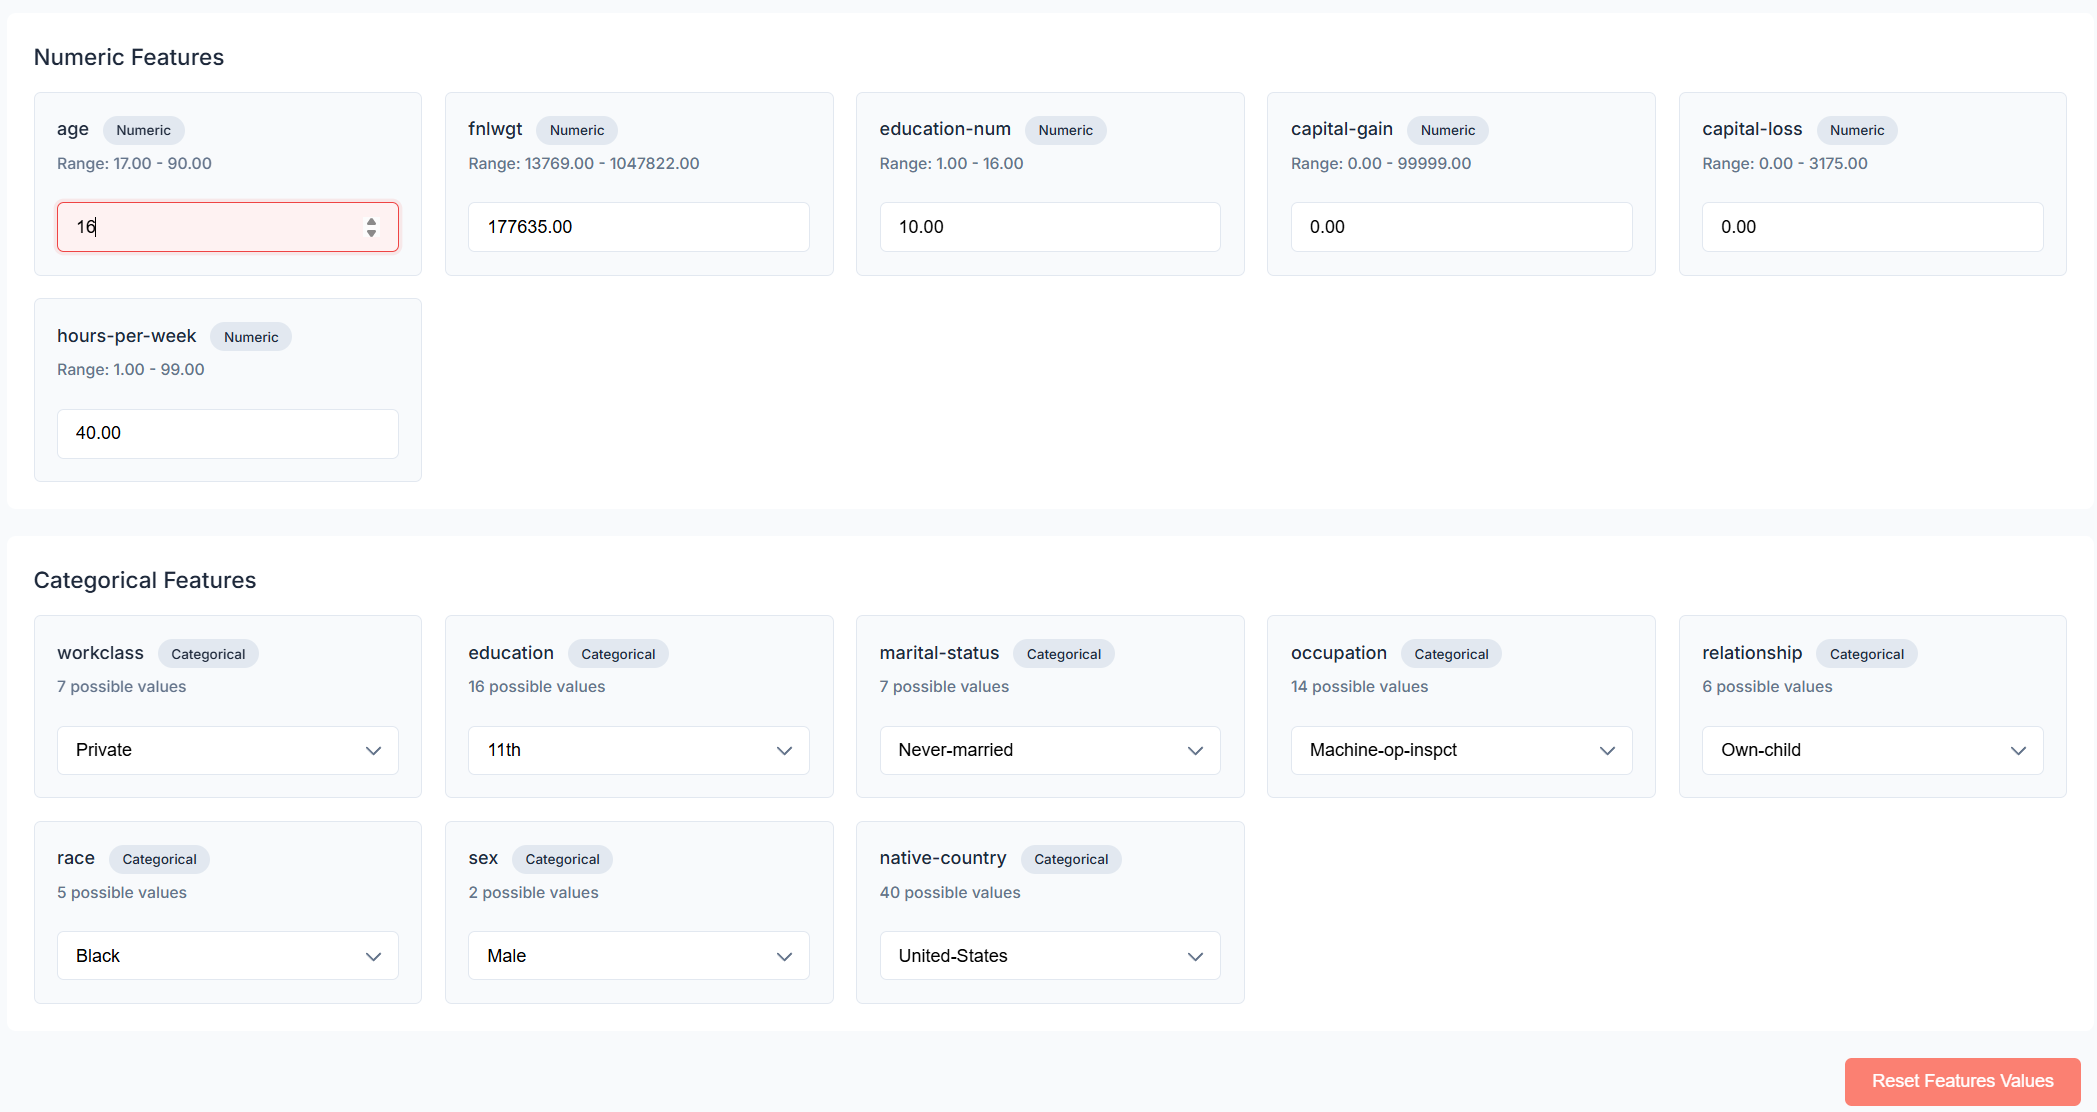
\includegraphics[width=0.9\textwidth]{images/featuresInputPanel.png}
  \caption{Feature input for the adult dataset with both numerical and categorical features and a out of bound input value for the feature "age".}
  \label{fig:featureInput}
\end{figure}

Following successful model training, the interface reveals the \textbf{instance feature input section}, shown in Figure \ref{fig:featureInput}, that enables users to specify the instance for which they seek an explanation. This component implements \textbf{adaptive input generation} that accommodates diverse feature types while maintaining intuitive interaction patterns.
% 
% \textbf{Feature Organization Strategy}: 
The interface organizes features into sections grouped by feature type: numeric features and categorical features. This organization reduces visual complexity for datasets with many features while maintaining logical grouping of data characteristics.
% 
% \textbf{Numeric Feature Inputs}: 
Numeric features receive \textbf{number input fields} with clearly displayed valid range information. Each input shows minimum and maximum acceptable values derived from training data characteristics, but still allows users to enter out-of-bounds values, showing at the same time when the value is out of bounds with a red highlight. The interface displays default values calculated as features median value, providing sensible starting points for exploration.
% 
% \textbf{Categorical Feature Inputs}: 
On the other hand,
categorical features utilize \textbf{dropdown select menus} populated with valid category values. The interface displays category options in a scrollable list. Default selections represent the mode value for the specific feature.

% \textbf{Reset Functionality}: 
A dedicated \textbf{"Reset Features Values" button} positioned above the feature sections enables users to restore all inputs to their default values, mean, and mode for either numerical or categorical features, facilitating exploration of different instance configurations without manual re-adjustment of each field.

\subsection{Explanation Parameters Settings}

\begin{figure}[htbp]
  \centering
  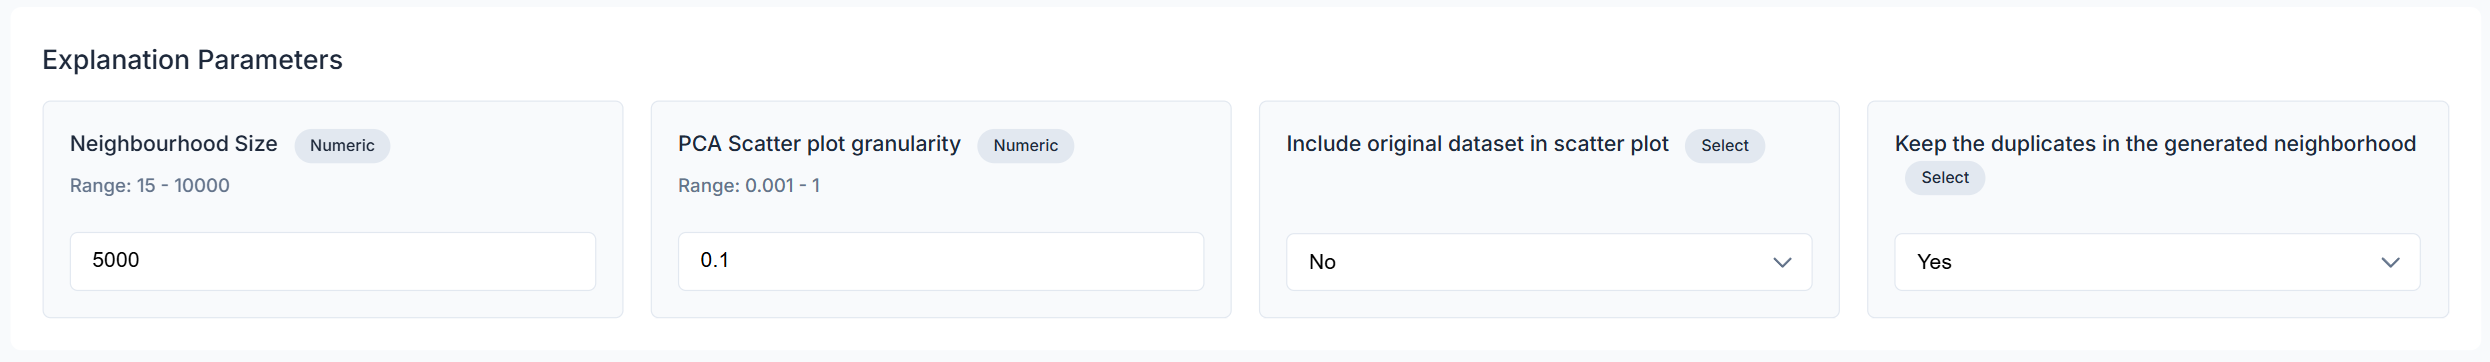
\includegraphics[width=0.9\textwidth]{images/ExplanationParameters.png}
  \caption{Explanation Parameters input.}
  \label{fig:ExplanationParameters}
\end{figure}

Below the feature input interface, the system presents the \textbf{"Explanation Parameters"} section, shown in Figure \ref{fig:ExplanationParameters}, which controls some $\text{LORE}_{sa}$ explanation generation parameters and visualization configuration settings.

\textbf{Neighbourhood Size}: The interface provides \textbf{numeric input controls} for synthetic neighborhood size, allowing users to specify the number of instances to generate around the explained instance. This parameter critically affects explanation quality, with larger neighborhoods providing more robust rule extraction at the cost of increased computational time.

\textbf{PCA Scatter plot granularity}: For PCA projections, the interface includes a \textbf{granularity control} that determines the resolution of Voronoi tessellation used for decision boundary visualization. Lower values create coarser approximations with better performance, while higher values produce more detailed boundary representations at increased computational cost.

\textbf{Include original dataset in scatter plot}: The interface provides a boolean toggle control that enables users to overlay the present original dataset onto the scatter plot visualization alongside the synthetic neighborhood. When enabled, original dataset points are rendered with reduced opacity to distinguish them from synthetic instances while providing crucial context about how the generated neighborhood relates to the broader data distribution. This feature facilitates assessment of neighborhood representativeness by enabling direct visual comparison between synthetic instances and actual training data patterns.

\textbf{Keep the duplicates in the generated neighborhood}: The interface includes thi boolean toggle control that determines whether the genetic algorithm's neighborhood generation process preserves or removes duplicate instances. When enabled, all generated instances are retained even if they have identical feature values, which may be relevant for analyzing the genetic algorithm's convergence behavior, but will increase the computational overhead in visualization rendering. 

\subsection{Dimensionality Reduction techniques Parameters Settings}

\begin{figure}[htbp]
  \centering
  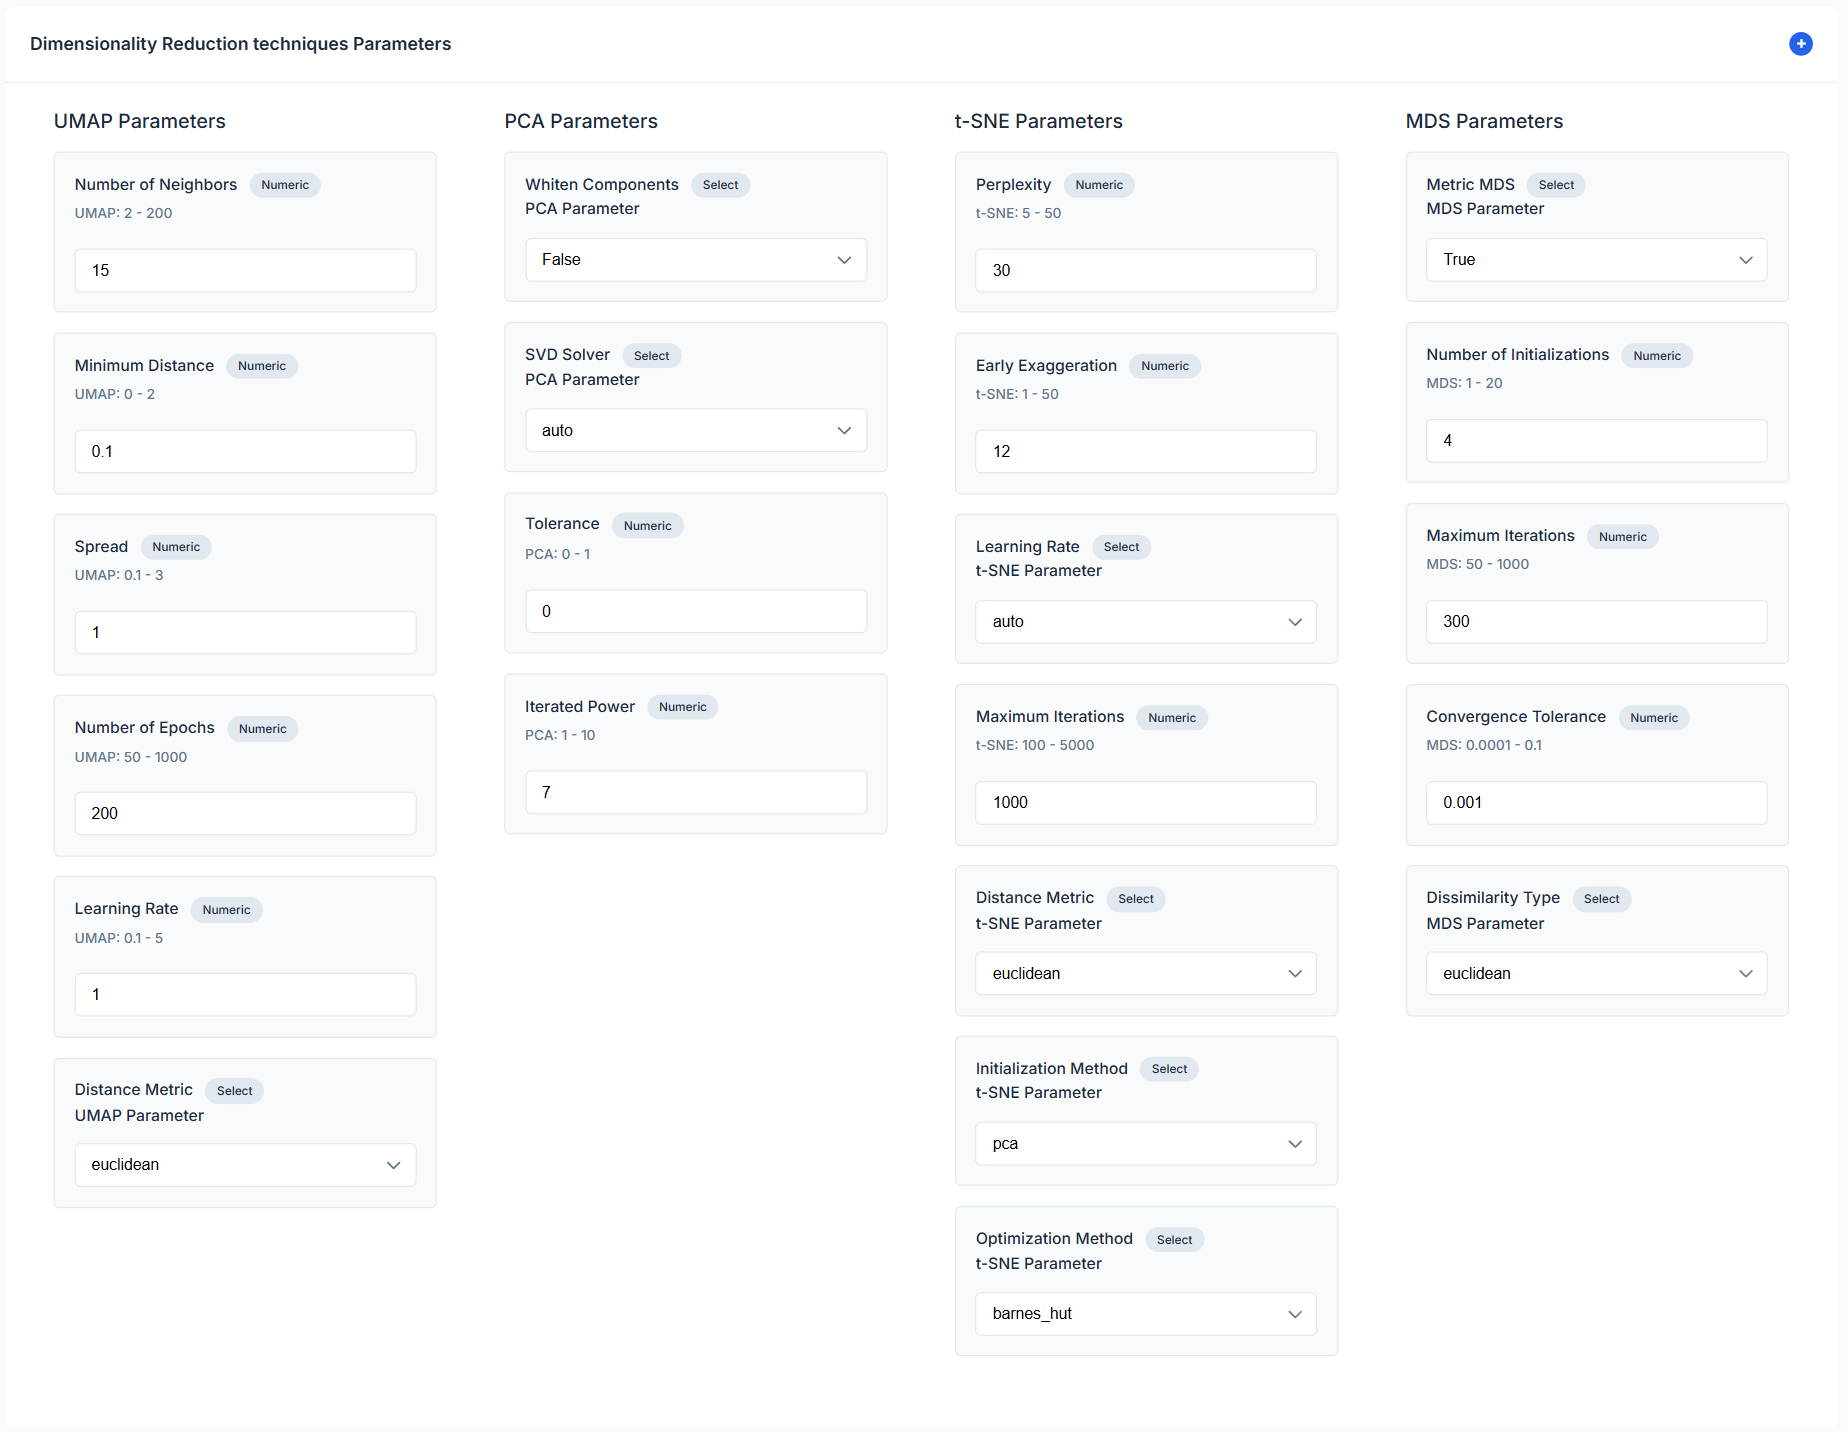
\includegraphics[width=0.9\textwidth]{images/Dimensionality Reduction Parameters.png}
  \caption{Dimensionality Reduction Parameters.}
  \label{fig:Dimensionality Reduction Parameters}
\end{figure}

The interface implements \textbf{expandable parameter sections} for each supported dimensionality reduction technique. Users can configure UMAP's `n\_neighbors` and `min\_dist` parameters, t-SNE's perplexity and learning rate, PCA's component selection, and MDS metric specifications and many other parameters for each of the dimensionality reduction techniques, as show in Figure \ref{fig:Dimensionality Reduction Parameters}. These advanced controls are presented in collapsible sections to avoid overwhelming novice users while remaining accessible to experts seeking fine-grained control.

\subsection{Visualization Selection Toggles}

\begin{figure}[htbp]
  \centering
  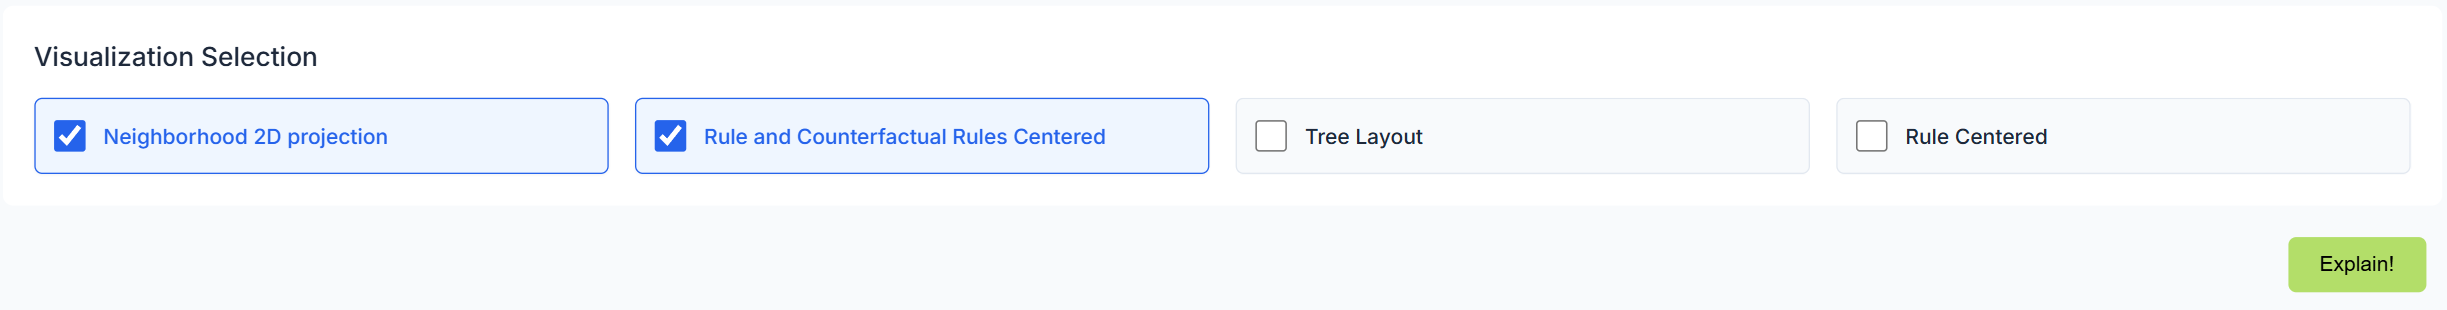
\includegraphics[width=0.9\textwidth]{images/Visualization Selection.png}
  \caption{Visualization Selection panel, allowing the user to choose which visualizations to render.}
  \label{fig:Visualization Selection}
\end{figure}

A critical component is the \textbf{visualization selection interface} that enables users to control which visualization components appear in the final explanation display. The interface presents \textbf{four checkbox toggles} corresponding to the Neighborhood 2D projection, Rule and Counterfactual Rules Centred surrogate model, Tree Layout surrogate model, and Rule Centered surrogate model visualizations.

% \textbf{Toggle Design}: 
Each visualization toggle employs a \textbf{checkbox with descriptive label} arranged in a grid layout. The toggles include visual indicators showing which visualizations are currently enabled, with checked boxes receiving enhanced styling through background color changes and border highlighting.
The Neighborhood 2D projection is, as previously said, selected by default and can not be deactivated, the user can then choose to render either of the three realized visualizations. The default selection is \texttt{Rule and Counterfactual Rules Centered}, and if the user chooses to select one of the other two the selection will behave as with an HTML ratio input.

% \textbf{Explanation Generation Trigger}: 
At the workflow conclusion, a the \textbf{"Explain!" button} starts the explanation generation. Upon click, the system displays an \textbf{animated loading interface} with progress indicators and descriptive text explaining the explanation generation process. This provides crucial user feedback during potentially lengthy operations involving genetic algorithm-based neighborhood generation and surrogate model training.

\section{Coordinated Visualization System}

Following successful explanation generation, the interface transitions to present the \textbf{coordinated visualization system} that displays the results through the two complementary views. The visualization system architecture centers on \textbf{coordinated multiple views} \cite{readingsInformationVi}, implementing two distinct but interconnected visualization components: the 2 dimensionality-reduced scatter plot for neighborhood exploration, and one of the three surrogate model visualizations that provide different points of view on the same surrogate model structure.

This multi-representation approach addresses the diverse cognitive approaches users may take when interpreting machine learning explanations. The visualization components appear below the configuration interface, maintaining access to configuration controls while presenting explanatory results.

The Bidirectional coordination serves as the fundamental interaction paradigm, enabling information flow between spatial and symbolic representations. Users can initiate interactions from any of the two visualization components, with the system automatically propagating highlighting and selection states across the other view. This coordination maintains visual consistency through synchronized color schemes and ensures that users can confirm explanations by cross-referencing between different representation modalities.

\section{2D spatial neighborhood analysis Visualization}


\begin{figure}[ht!]
    \centering
    \begin{subfigure}[c]{0.68\textwidth}
        \centering
        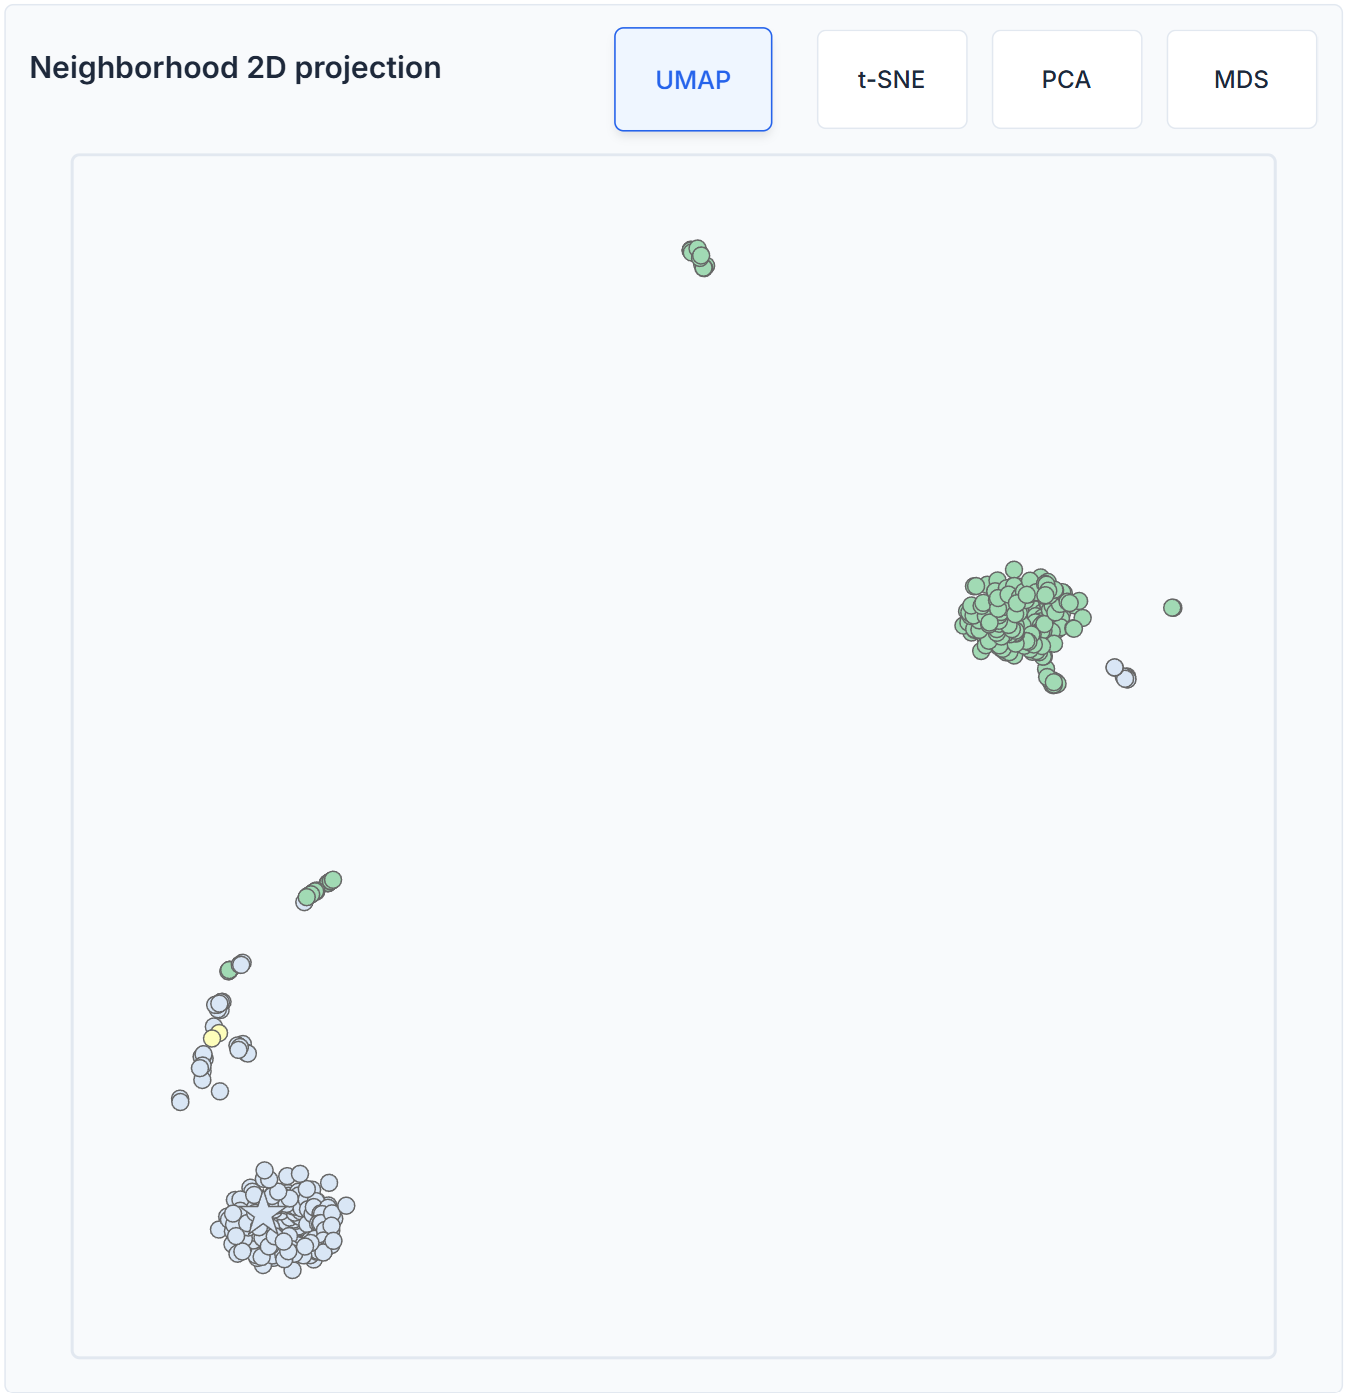
\includegraphics[width=\textwidth]{images/scatterPlotFinal.png}
        \caption{Example of generated spatial neighborhood analysis plot.}
        \label{fig:scatterPlotFinal}
    \end{subfigure}
    \hfill
    \begin{subfigure}[c]{0.28\textwidth}
        \centering
        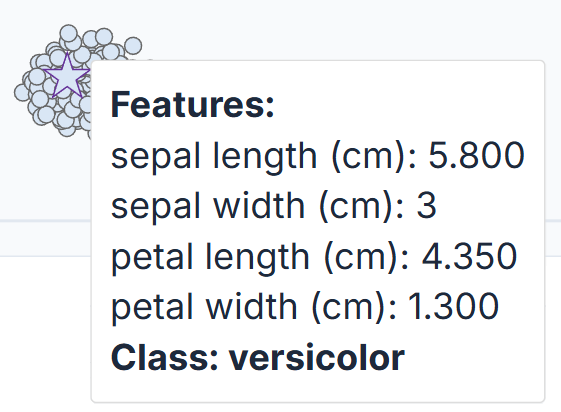
\includegraphics[width=\textwidth]{images/scatterPlotFinalHover.png}
        \caption{Example of hover on a spatial neighborhood analysis plot point.}
        \label{fig:scatterPlotFinalHover}
    \end{subfigure}

    \caption{Generated spatial neighborhood analysis plot.}
\end{figure}

The spatial neighborhood analysis plot component, example of which is shown in Figure \ref{fig:scatterPlotFinal}, represents the spatial interface for exploring the synthetic neighborhood, serving as the primary mechanism for understanding the quality and distribution of generated instances in reduced-dimensional space. The implementation supports four distinct dimensionality reduction techniques, each accessible through radio button controls integrated directly into the visualization header.

% \textbf{Dimensionality Reduction Integration}: 
The interface provides the switching mechanism between \textbf{Uniform Manifold Approximation and Projection (UMAP)}, \textbf{t-distributed Stochastic Neighbor Embedding (t-SNE)}, \textbf{Principal Component Analysis (PCA)}, and \textbf{Multidimensional Scaling (MDS)}. Each method offers distinct advantages for different analytical scenarios.
The radio button controls appear immediately above the spatial neighborhood analysis plot, enabling rapid switching between projection methods without requiring navigation away from the visualization context. 

% \textbf{Visual Encoding Strategy}: 
The spatial neighborhood analysis plot employs a sophisticated multi-layered visual encoding approach that maximizes information density while maintaining clarity. \textbf{Point symbols} distinguish between synthetic neighborhood instances (circles) and the explained instance (star), with symbol size differentiation ensuring the explained instance remains clearly identifiable within the neighborhood context. \textbf{Color encoding} employs a perceptually uniform color scheme projected from the CIELAB color space, ensuring consistent class differentiation across varying numbers of target categories.
%
Opacity-based differentiation addresses the challenge of displaying both original dataset points and synthetic neighborhood instances within the same visualization space. Original dataset points are rendered with reduced opacity, creating a contextual background that helps users understand how the synthetic neighborhood relates to the broader data distribution without overwhelming the primary explanation content.

% \textbf{Decision Boundary Visualization}: 
For linear transformations (PCA), the system implements \textbf{Voronoi tessellation-based decision boundaries} that provide explicit visualization of classification regions within the projected space. The Voronoi implementation employs user-configurable granularity settings (controlled through the Surrogate Model Parameters section), allowing adjustment of boundary precision based on computational constraints and visualization clarity requirements. Semi-transparent polygon regions use class-consistent coloring to create intuitive decision boundary representations that enable direct assessment of explanation quality through boundary geometric properties.

% \textbf{Interactive Capabilities}: 
The spatial neighborhood analysis plot supports comprehensive interaction mechanisms designed to facilitate explanation exploration. \textbf{Zoom and pan functionality} enables detailed examination of neighborhood regions, with smooth transitions maintaining spatial orientation. The zoom implementation preserves aspect ratios and provides intuitive mouse wheel or pinch-to-zoom interactions.
%
The hover interactions, example of which is shown in Figure \ref{fig:scatterPlotFinalHover}, reveal detailed point information through contextual tooltips that display decoded feature values, class predictions, and positional coordinates. The tooltips follow cursor movement smoothly and employ \textbf{details-on-demand} principles \cite{readingsInformationVi}, appearing only when needed to avoid visual clutter.
%
The point selection interactions serve as the primary mechanism for triggering cross-visualization coordination. Clicking any point initiates highlighting of the corresponding decision path in the selected tree visualization, while simultaneously highlighting the selected point with a distinct color. 
Clicking the same point again deselects it and clears all highlighting, providing intuitive toggle behavior.

\section{Tree Layout Visualization}

\begin{figure}[ht!]
    \centering
    \begin{subfigure}[c]{0.68\textwidth}
        \centering
        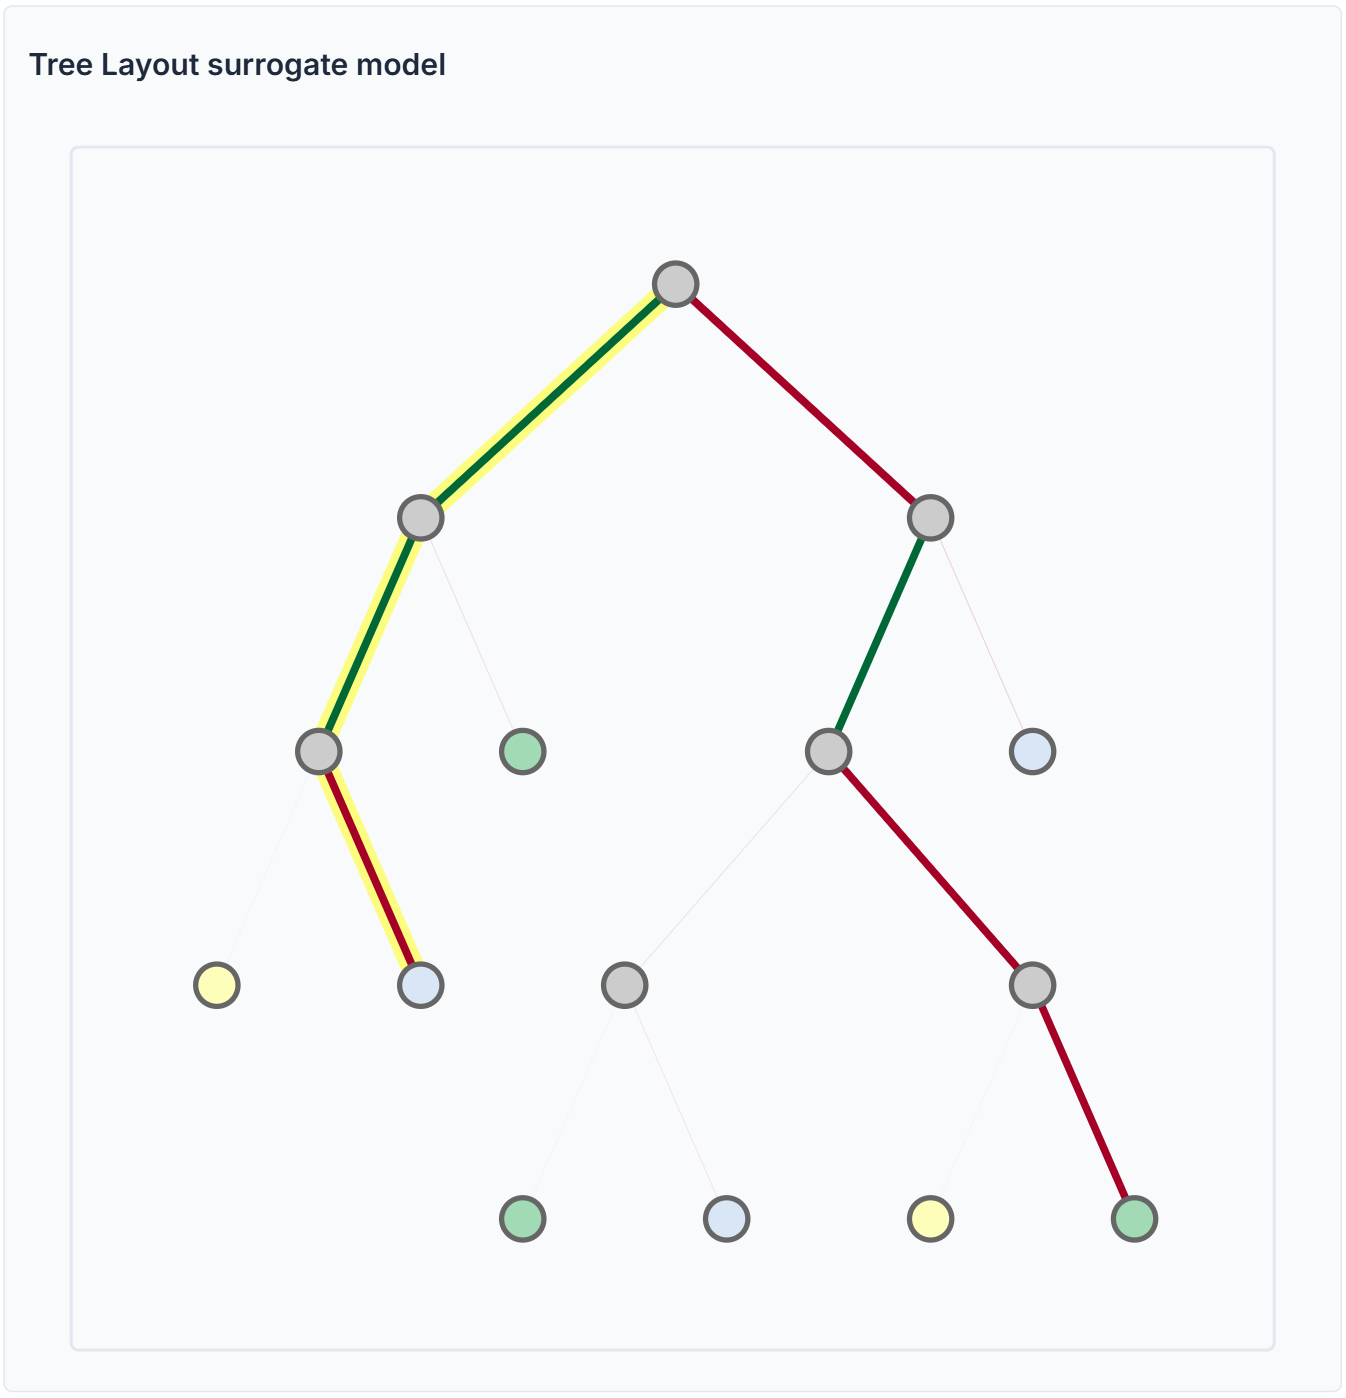
\includegraphics[width=\linewidth]{images/classicalDecisionTreeFinal.png}
        \caption{Tree Layout visualization.}
        \label{fig:classicDecisionTreeFinal}
    \end{subfigure}%
    \hfill
    \begin{subfigure}[c]{0.28\textwidth}
        \centering
        \begin{subfigure}[c]{\linewidth}
            \centering
            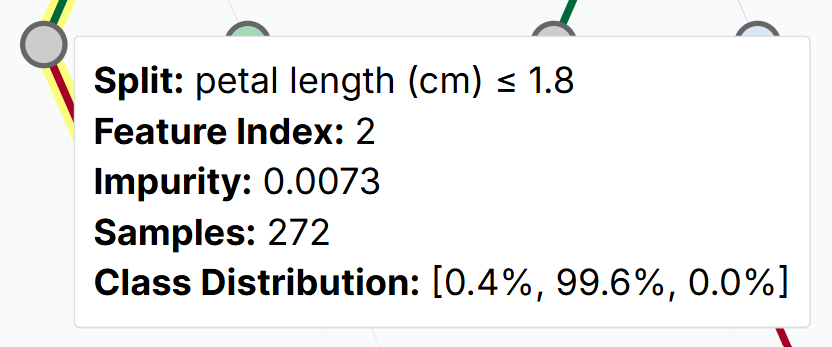
\includegraphics[width=\linewidth]{images/classicalDecisionTreeFinalTooltipSplit.png}
            \caption{Tooltip on the Tree Layout visualization for a split node}
            \label{fig:classicalDecisionTreeFinalTooltipSplit}
        \end{subfigure}
        \vspace{1cm}
        \begin{subfigure}[c]{\linewidth}
            \centering
            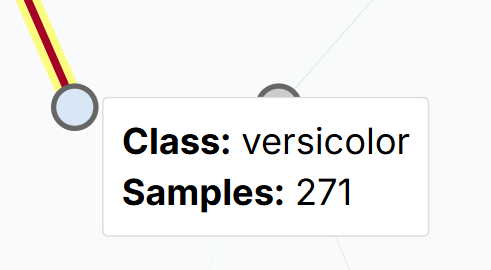
\includegraphics[width=\linewidth]{images/classicalDecisionTreeFinalTooltipLeaf.png}
            \caption{Tooltip on the Tree Layout visualization for a leaf node}
            \label{fig:classicalDecisionTreeFinalTooltipLeaf}
        \end{subfigure}
    \end{subfigure}
    
    \caption{Tree Layout visualization and tooltips.}
\end{figure}

The Tree Layout visualization, shown in Figure \ref{fig:classicDecisionTreeFinal}, provides the foundational hierarchical representation of the surrogate model, implementing established node-link diagram conventions while incorporating interaction capabilities. This visualization serves as a primary reference for understanding logical rule structure and decision flow.

% \textbf{Node-Link Layout}: 
The implementation employs a \textbf{traditional top-down hierarchical layout} with systematic node positioning that prevents overlapping while maintaining clear parent-child relationships. \textbf{Circular nodes} represent decision points and leaves.
% 
% \textbf{Visual Encoding System}: 
The color encoding strategy distinguishes between split nodes and leaf nodes through coordinated class-based coloring. \textbf{Split nodes} (representing logical conditions) employ neutral gray coloring to emphasize their decision-making role without competing with class-specific colors. \textbf{Leaf nodes} receive coloring that directly corresponds to their predicted class, using the same color scheme employed in the spatial neighborhood analysis visualization to maintain cross-visualization consistency.
%
Edge visualization uses variable stroke width encoding to represent the flow of synthetic instances through decision branches. Thicker edges indicate paths with more instances, providing immediate visual feedback about decision tree utilization patterns. 
The edges also visually encode which split outcome they pursue, with negative ramification being red and green for the opposite case.

Tooltip information provides comprehensive contextual details through details-on-demand interaction. Split node tooltips, shown in Figure \ref{fig:classicalDecisionTreeFinalTooltipSplit}, reveal feature names, threshold values, impurity measures (Gini or entropy), sample counts, and class distribution statistics. Leaf node tooltips, shown in Figure \ref{fig:classicalDecisionTreeFinalTooltipLeaf}, display class prediction and sample counts. This layered information approach allows users to access varying levels of detail based on their analytical requirements.

\begin{figure}
    \centering
    \begin{subfigure}[c]{0.48\textwidth}
        \centering
        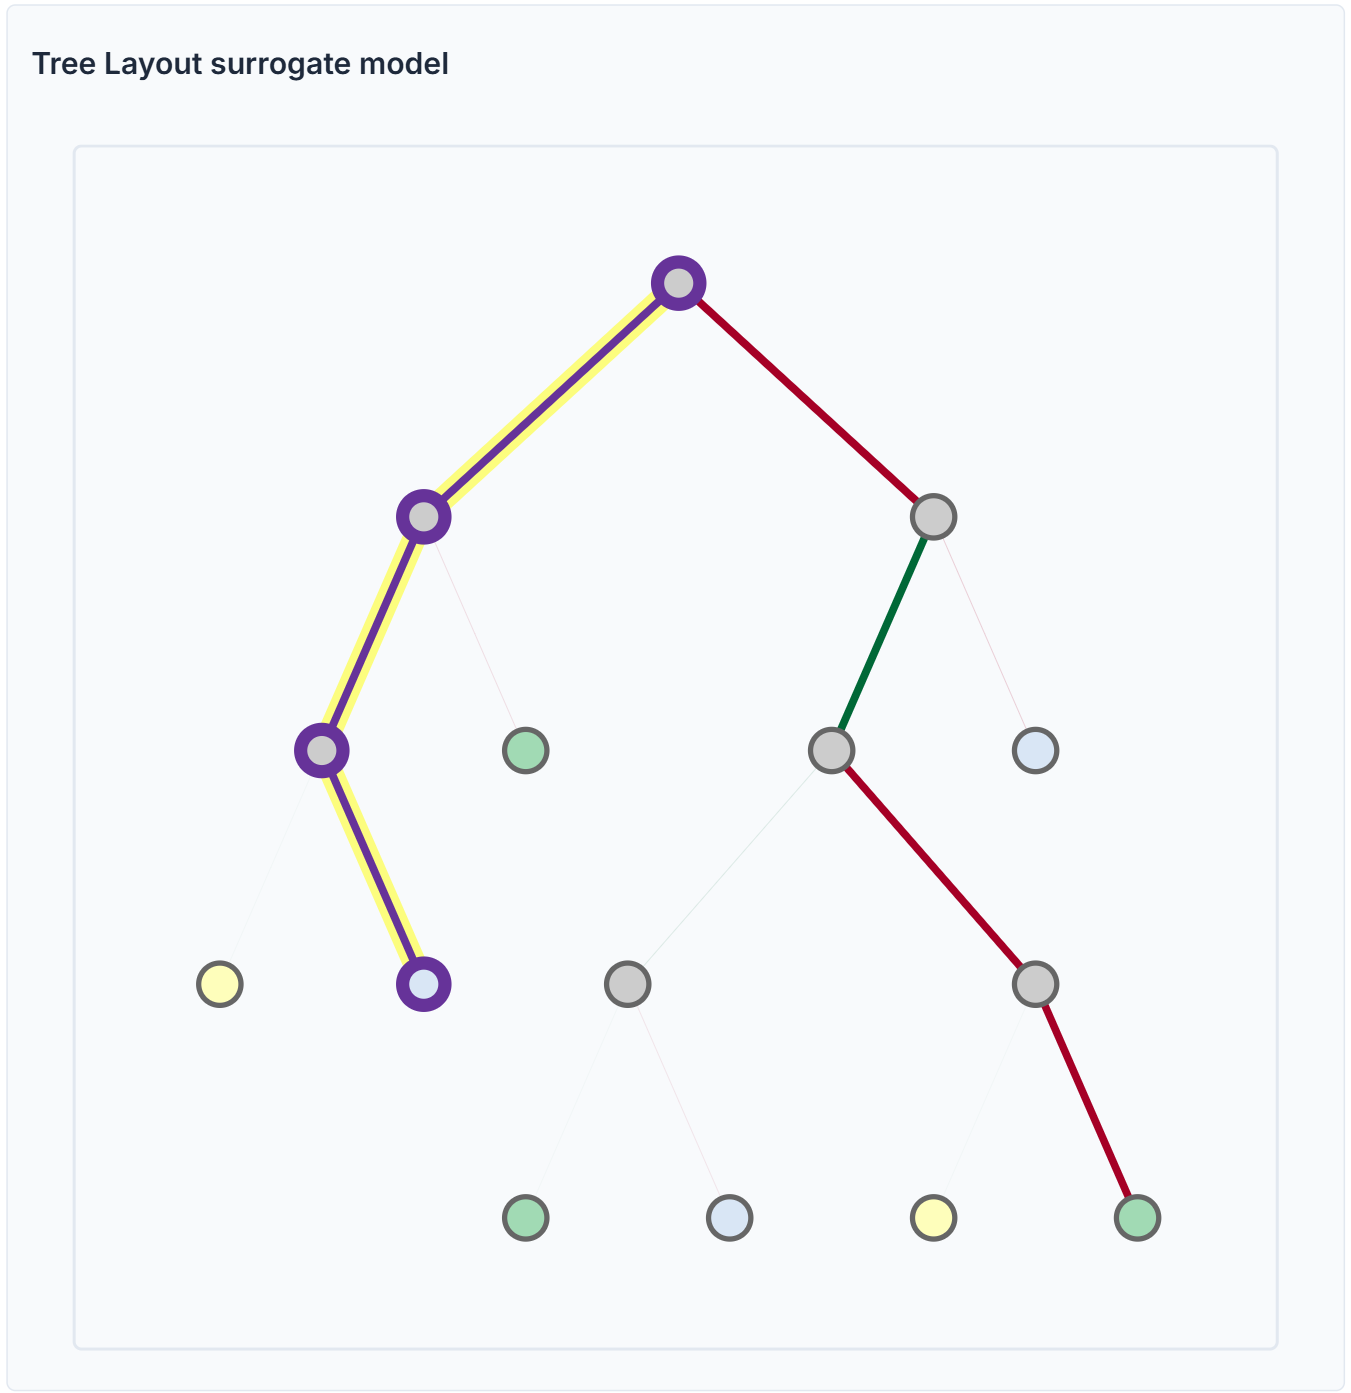
\includegraphics[width=\linewidth]{images/classicalDecisionTreeFinalLeafInteraction.png}
        \caption{Click on leaf node interaction.}
        \label{fig:classicDecisionTreeFinalLefClick}
    \end{subfigure}
    \vspace{0.3cm}
    \begin{subfigure}[c]{0.48\linewidth}
        \centering
        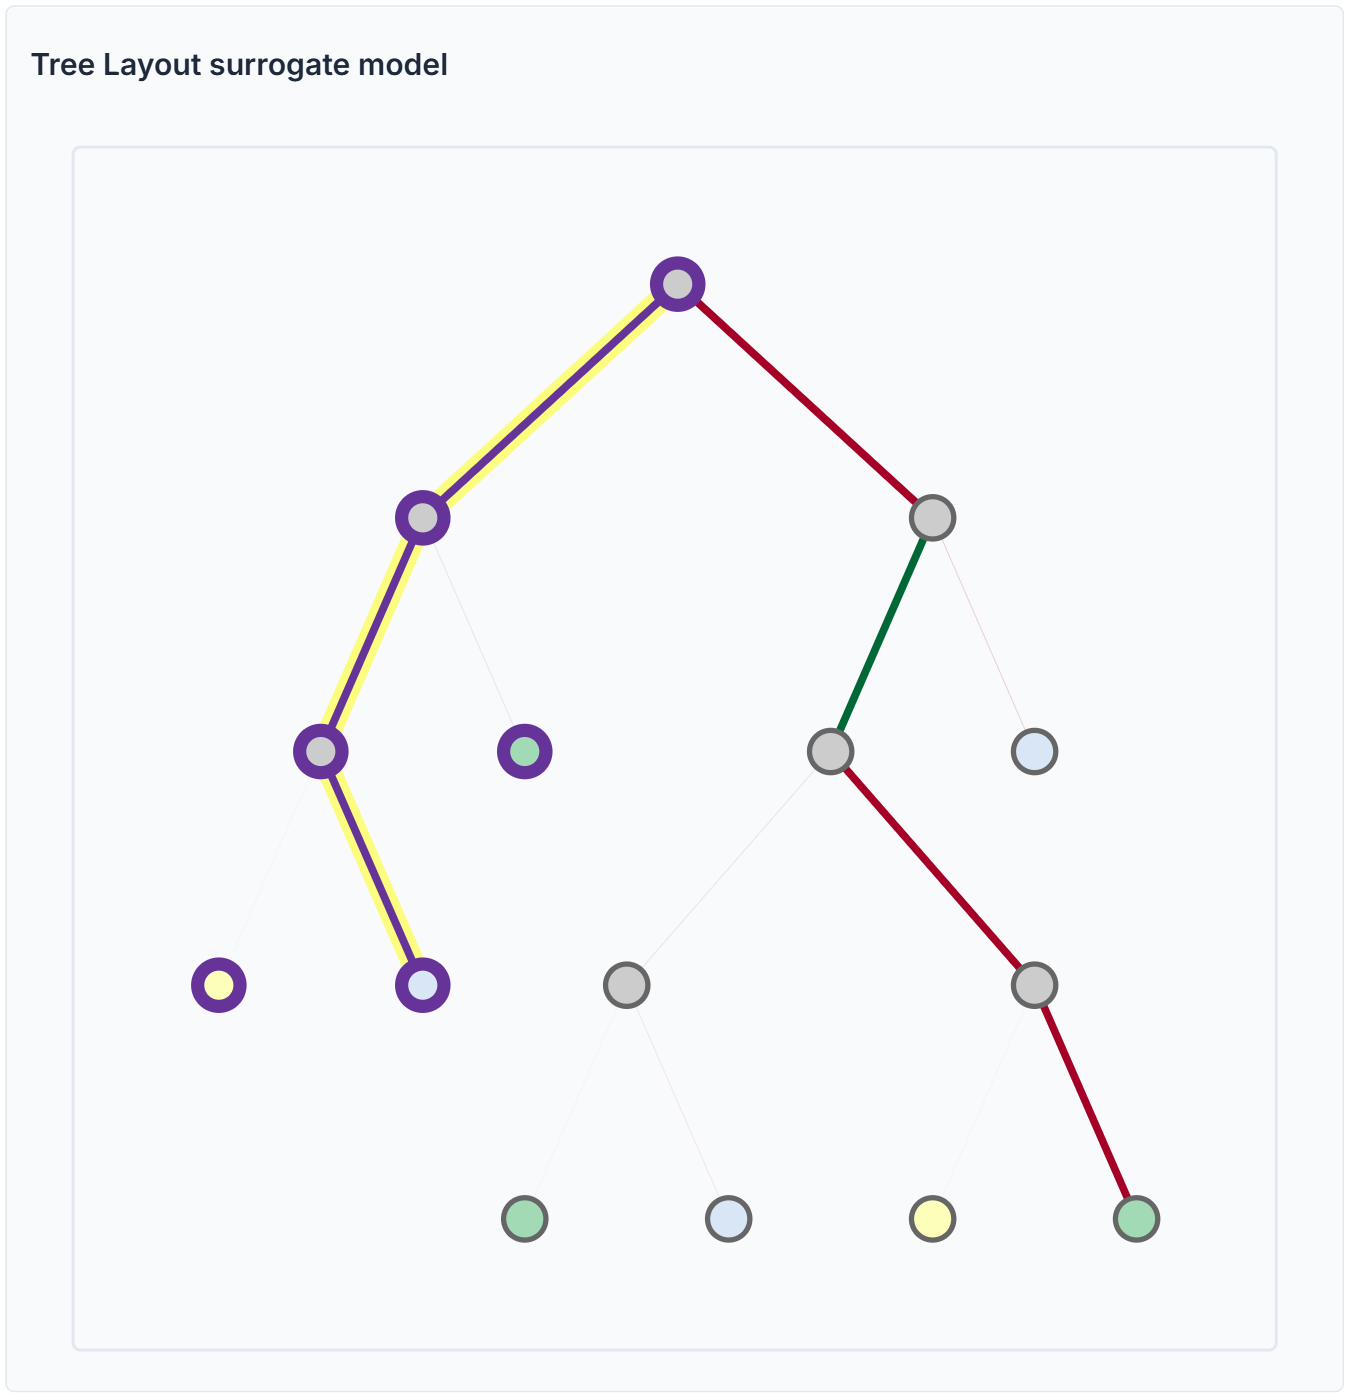
\includegraphics[width=\linewidth]{images/classicalDecisionTreeFinalSplitInteraction.png}
        \caption{Click on split node interaction.}
        \label{fig:classicDecisionTreeFinalSplitClick}
    \end{subfigure}
    \caption{Classical decision tree click interactions.}
\end{figure}

% \textbf{Interaction Architecture}: 
The Tree Layout visualization implements interaction mechanisms that coordinate with all other visualization components. \textbf{Node click interactions} trigger highlighting of corresponding instances in the spatial neighborhood analysis plot, with leaf node clicks, showcased in Figure \ref{fig:classicDecisionTreeFinalLefClick}, highlighting all instances satisfying the complete logical path, and split node clicks, showcased in Figure \ref{fig:classicDecisionTreeFinalSplitClick}, highlighting instances passing through specific decision points.
%
Path highlighting provides persistent visual feedback for explained instance trajectories through the tree. The explained instance's path from root to leaf receives continuous highlighting using stroke width enhancement and color differentiation, ensuring users can easily trace the logical conditions that led to the specific prediction.

% \textbf{Zoom and Pan}: 
The Tree Layout visualization includes \textbf{interactive zoom and pan capabilities} that enable detailed examination of complex tree structures. Users can mouse-wheel zoom or use trackpad gestures to adjust magnification levels, with the system maintaining tree center positioning and providing smooth interpolation between zoom states.

\section{Rule and Counterfactual Rules Centered Visualization}

\begin{figure}[ht!]
    \centering
    \begin{subfigure}[c]{0.68\textwidth}
        \centering
        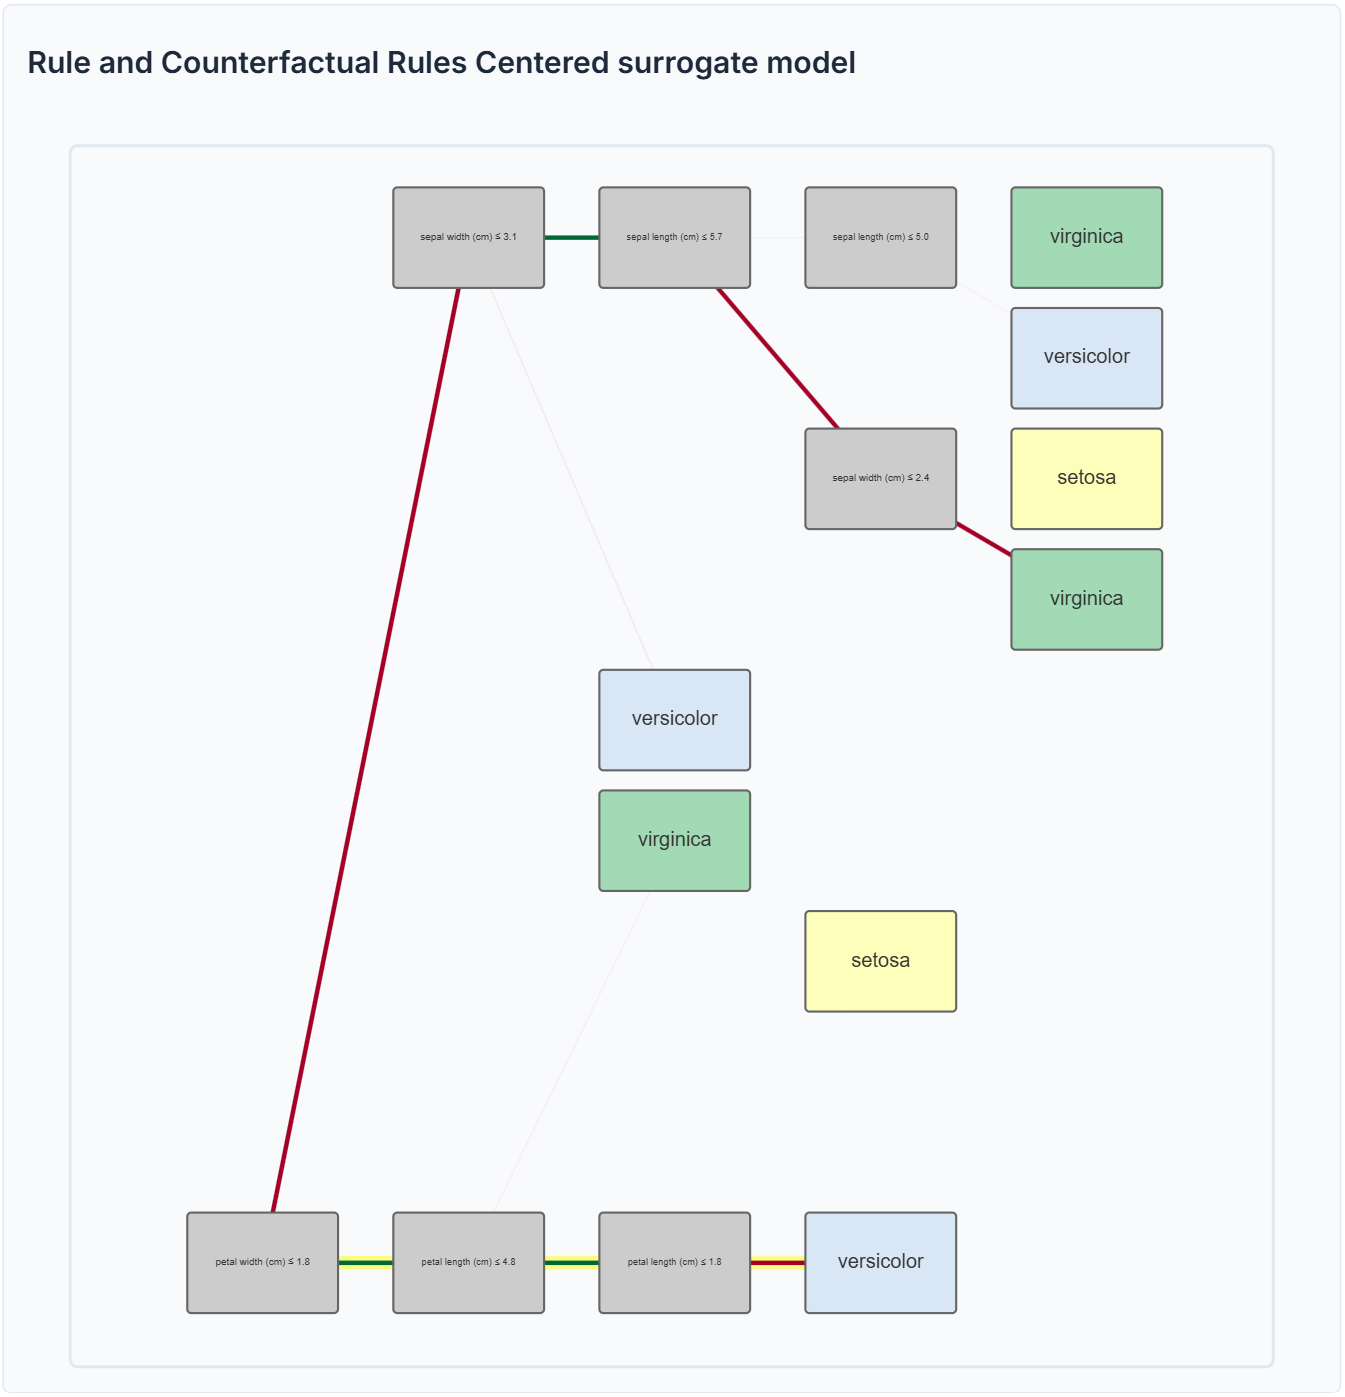
\includegraphics[width=\linewidth]{images/blocksPlotFinal.png}
        \caption{Rule and Counterfactual Rules Centered plot.}
        \label{fig:blocksDecisionTreeFinal}
    \end{subfigure}%
    \hfill
    \begin{subfigure}[c]{0.28\textwidth}
        \centering
        \begin{subfigure}[c]{\linewidth}
            \centering
            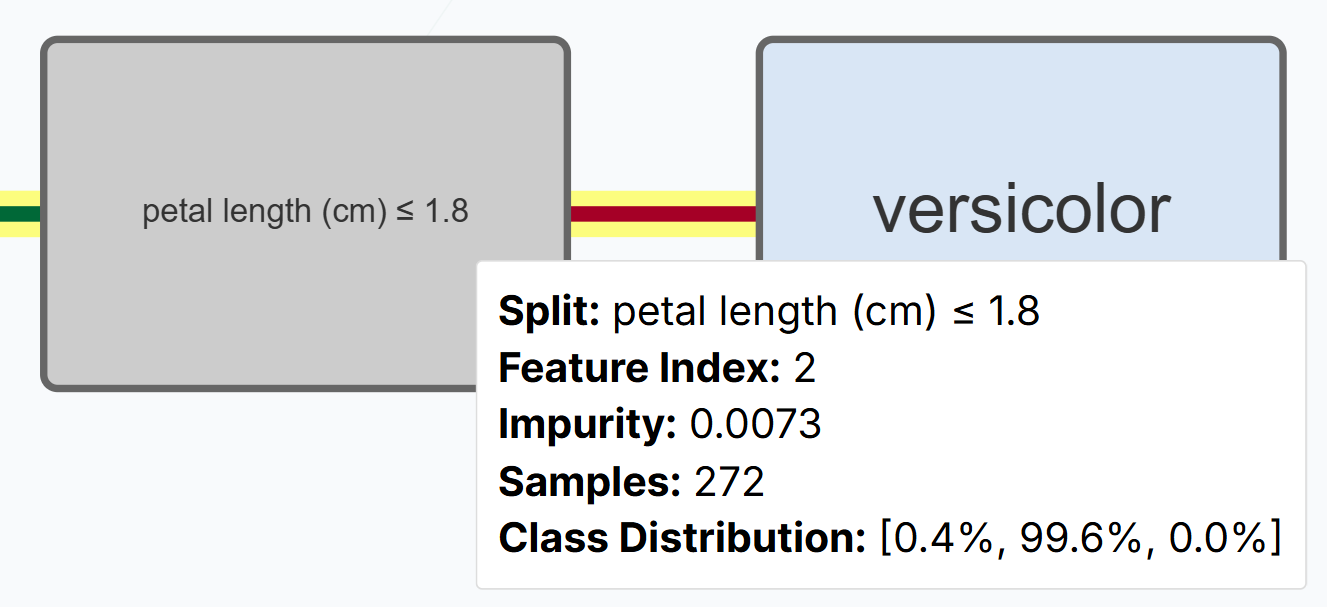
\includegraphics[width=\linewidth]{images/blocksDecisionTreeFinalTooltipSplit.png}
            \caption{Tooltip on the Rule and Counterfactual Rules Centered visualization for a split node}
            \label{fig:blocksDecisionTreeFinalTooltipSplit}
        \end{subfigure}
        \vspace{1cm}
        \begin{subfigure}[c]{\linewidth}
            \centering
            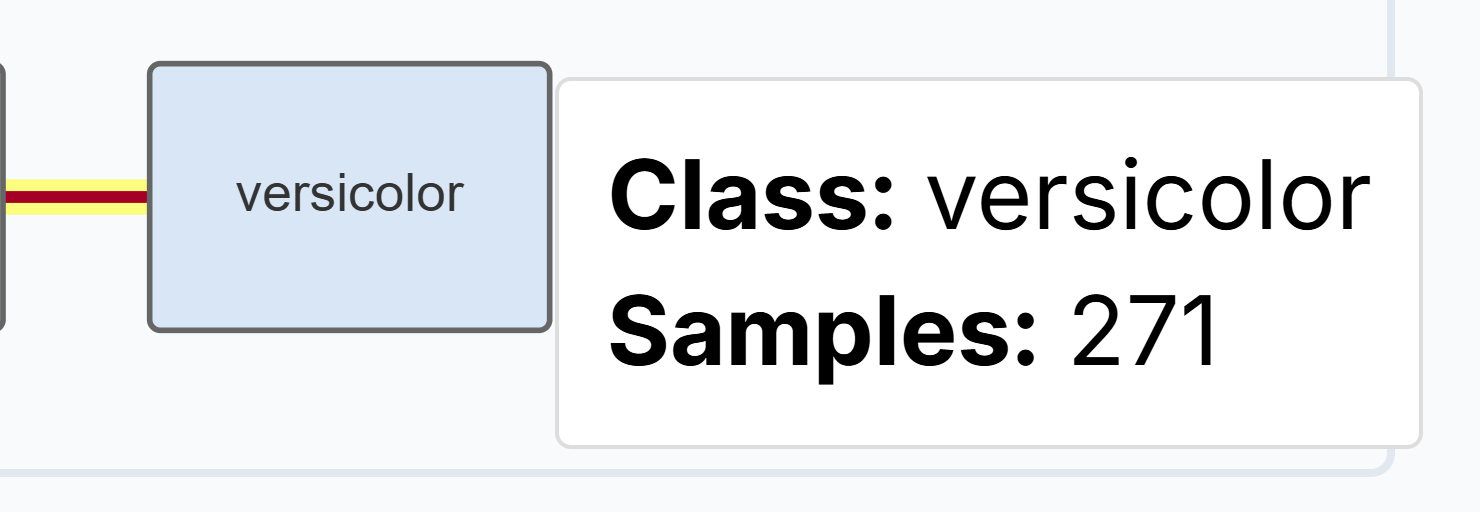
\includegraphics[width=\linewidth]{images/blocksDecisionTreeFinalTooltipLeaf.png}
            \caption{Tooltip on the Rule and Counterfactual Rules Centered visualization for a leaf node}
            \label{fig:blocksDecisionTreeFinalTooltipLeaf}
        \end{subfigure}
    \end{subfigure}
    
    \caption{Rule and Counterfactual Rules Centered visualization and tooltips.}
\end{figure}

The Rule and Counterfactual Rules Centered visualization, shown in Figure \ref{fig:blocksDecisionTreeFinal}, represents an innovative approach to hierarchical visualization that addresses layout efficiency challenges inherent in traditional node-link diagrams. This visualization employs \textbf{rectangular node representations} with \textbf{depth-aligned positioning} to create more compact and readable tree layouts, particularly effective for complex decision structures.

% \textbf{Depth-Aligned Layout Strategy}: 
Unlike traditional tree layouts that position nodes based on hierarchical relationships with varying vertical spacing, the Rule and Counterfactual Rules Centered visualization employs \textbf{horizontal depth alignment} where all nodes at the same tree depth occupy the same vertical level. This approach creates a more structured, grid-like appearance that facilitates comparison of decision complexity across different tree levels. 
% 
% \textbf{Explained Instance Path Emphasis}: 
A key design feature of the Rule and Counterfactual Rules Centered visualization the \textbf{guaranteed bottom positioning of the explained instance path}. This path in the tree is always rendered at the bottom of the visualization; therefore users can quickly locate the specific decision path of the generated rule, focusing their attention on the bottom region of the display. This consistent spatial organization reduces visual search time and cognitive load, particularly when exploring alternative decision paths.

% \textbf{Rectangular Node Design}: 
\textbf{Rectangular nodes} replace circular representations to maximize information density while improving text readability. Node dimensions adapt dynamically to accommodate textual content, with font sizing automatically adjusting to maintain readability across varying node sizes. Split nodes display decision conditions clearly within the rectangular bounds, while leaf nodes prominently feature class predictions and sample count information.
% 
% \textbf{Link Visualization}: 
\textbf{Straight-line connections} between rectangular nodes provide clear, unambiguous path representation. Variable stroke width encoding continues to represent instance flow, with stroke width proportional to the number of samples traversing each edge. \textbf{Color-coded edges} distinguish between "true" (left) and "false" (right) decision paths, using the same consistent color scheme employed across all visualizations.

% \textbf{Tooltip Information}: 
The blocks tree provides comprehensive contextual details through details-on-demand interaction, matching the Tree Layout visualization. Split node tooltips, shown in Figure \ref{fig:blocksDecisionTreeFinalTooltipSplit}, reveal feature names, threshold values, impurity measures, sample counts, and class distribution statistics within the rectangular node format. Leaf node tooltips, shown in Figure \ref{fig:blocksDecisionTreeFinalTooltipLeaf}, display class distributions, confidence measures, and sample counts, maintaining consistency with the classic tree's information architecture.

\begin{figure}
    \centering
    \begin{subfigure}[c]{0.48\textwidth}
        \centering
        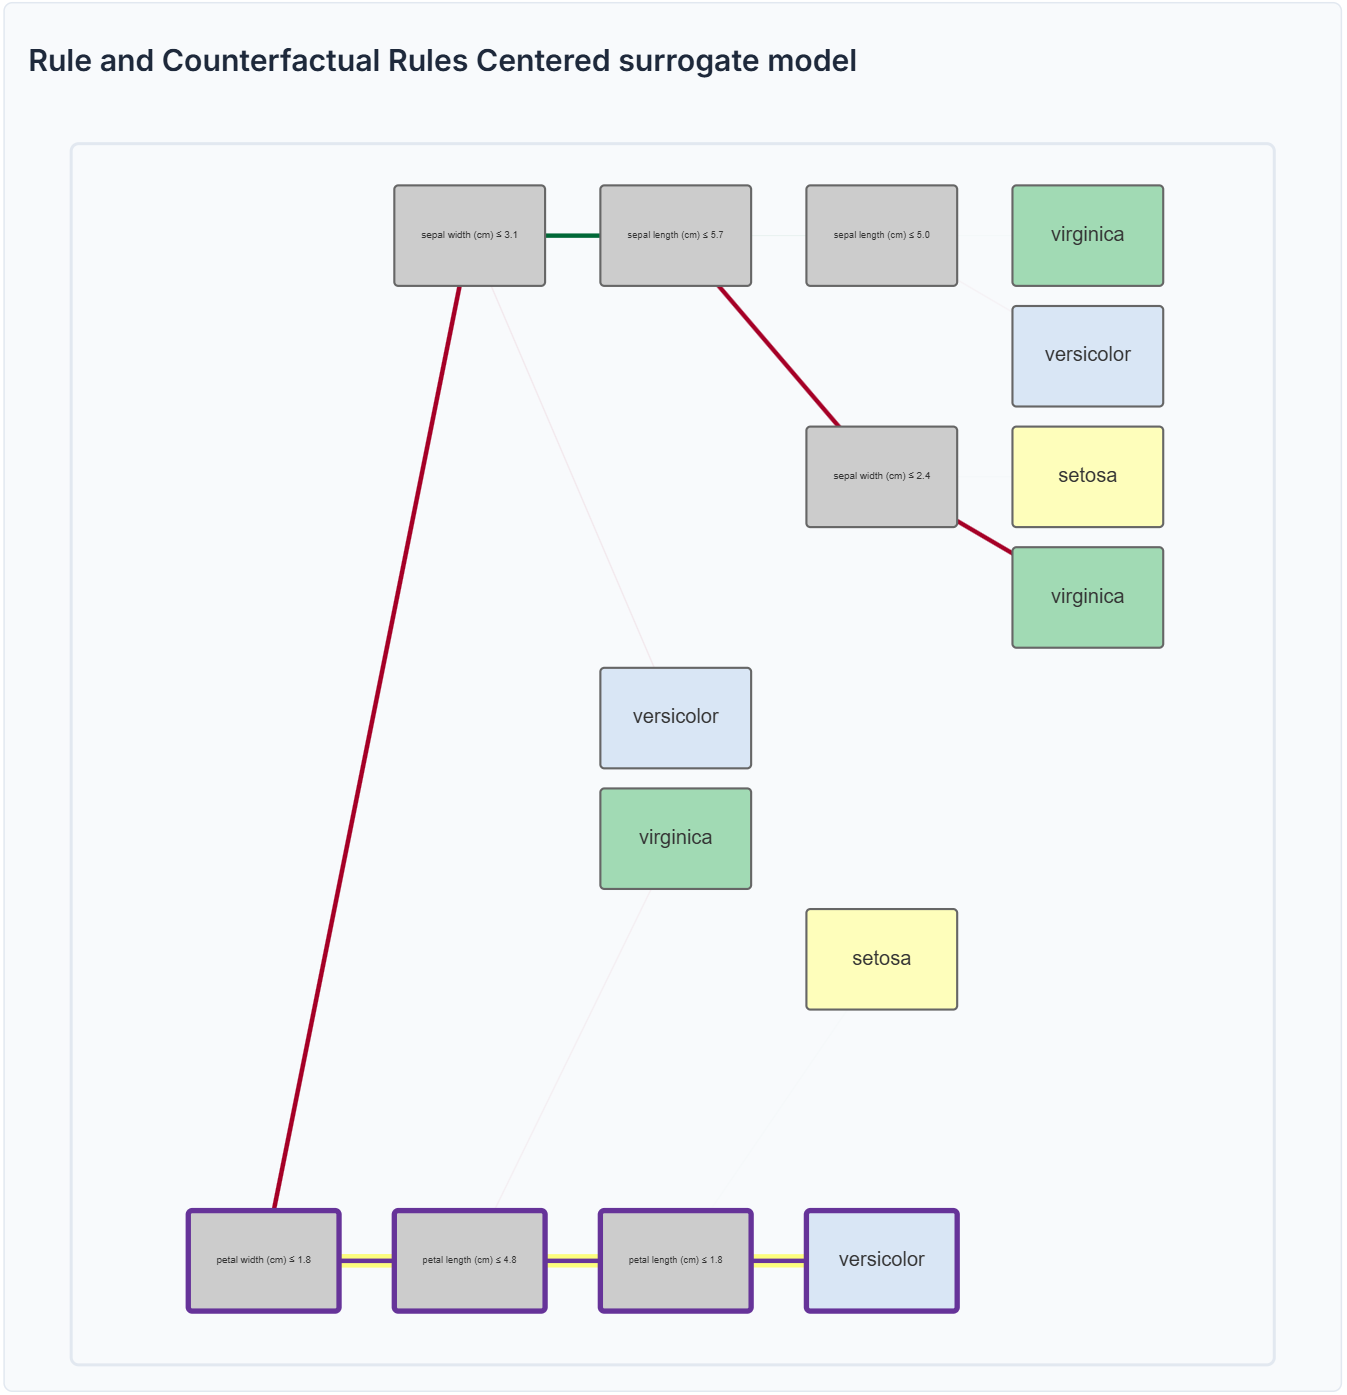
\includegraphics[width=\linewidth]{images/blocksDecisionTreeFinalLeafInteraction.png}
        \caption{Click on leaf node interaction.}
        \label{fig:blocksDecisionTreeFinalLeafClick}
    \end{subfigure}
    \vspace{0.3cm}
    \begin{subfigure}[c]{0.48\linewidth}
        \centering
        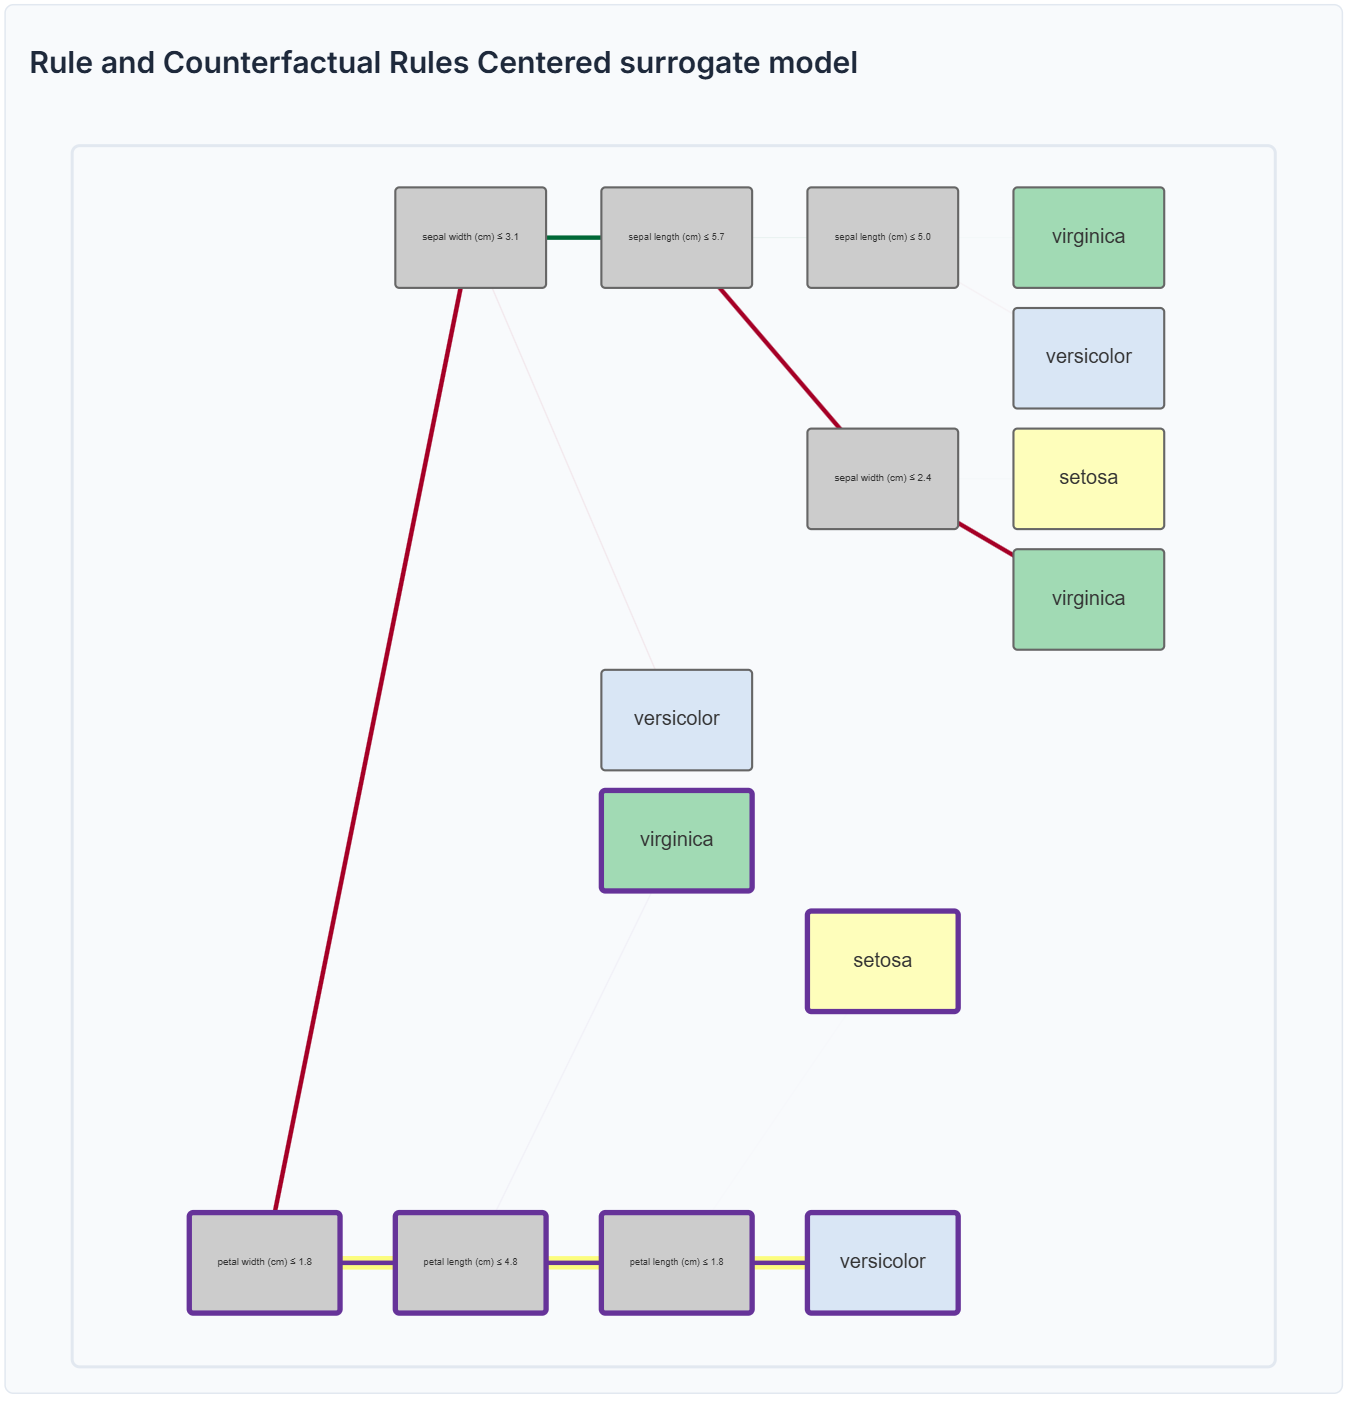
\includegraphics[width=\linewidth]{images/blocksDecisionTreeFinalSplitInteraction.png}
        \caption{Click on split node interaction.}
        \label{fig:blocksDecisionTreeFinalSplitClick}
    \end{subfigure}
    \caption{Blocks decision tree click interactions.}
\end{figure}

% \textbf{Coordinated Highlighting}: 
The Rule and Counterfactual Rules Centered visualization implements the same bidirectional coordination mechanisms as the Tree Layout visualization, with node interactions triggering corresponding highlights in the spatial neighborhood analysis plot and other tree visualizations. \textbf{Rectangle selection}, demonstrated in Figures \ref{fig:blocksDecisionTreeFinalLeafClick} and \ref{fig:blocksDecisionTreeFinalSplitClick}, provides more generous interaction targets compared to circular nodes, improving usability particularly for complex trees with many small nodes. Leaf node clicks highlight all instances satisfying the complete logical path, while split node clicks highlight instances passing through specific decision points.

% \textbf{Information Integration}: 
The rectangular format enables more effective integration of statistical information within node representations. Sample counts, impurity measures, and class distributions can be displayed more prominently within rectangular bounds, reducing reliance on tooltip interactions for frequently accessed information. This design decision reflects the principle of making important information directly visible rather than requiring interaction to access it.

\section{Rule Centered visualization}

\begin{figure}[ht!]
    \centering
    \begin{subfigure}[c]{0.68\textwidth}
        \centering
        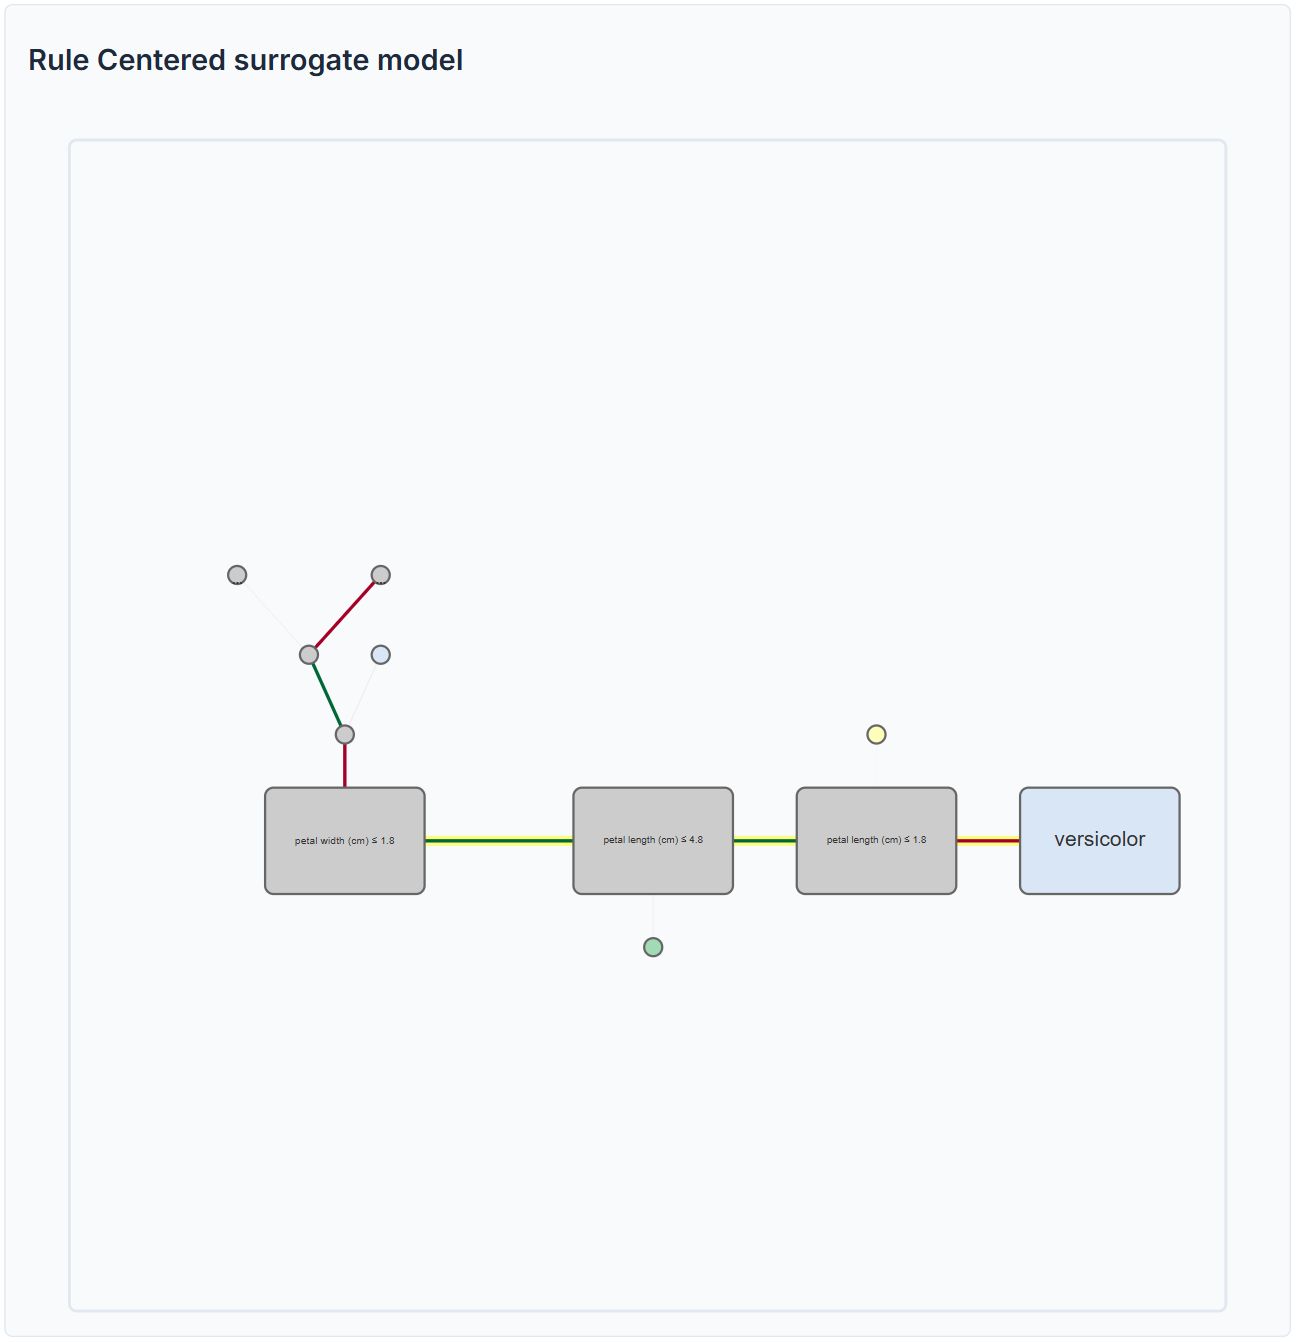
\includegraphics[width=\linewidth]{images/spawnPlotFinal.png}
        \caption{Rule Centered visualization plot.}
        \label{fig:spawnDecisionTreeFinal}
    \end{subfigure}%
    \hfill
    \begin{subfigure}[c]{0.28\textwidth}
        \centering
        \begin{subfigure}[c]{\linewidth}
            \centering
            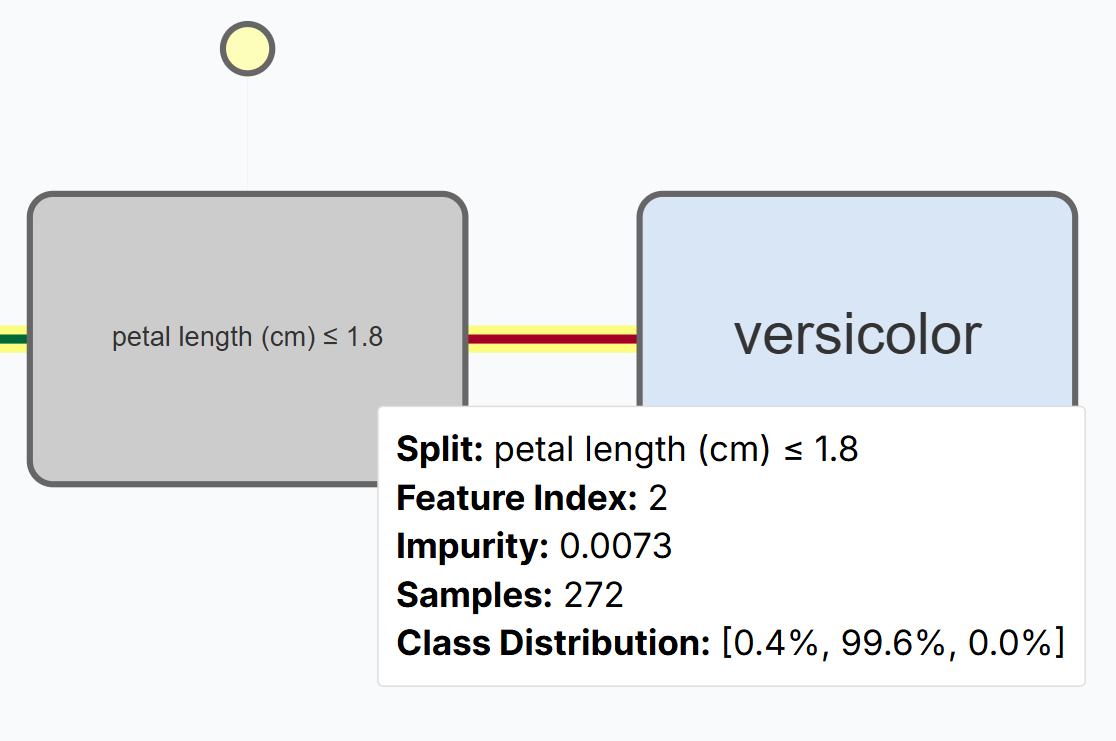
\includegraphics[width=\linewidth]{images/spawnDecisionTreeFinalTooltipSplit.png}
            \caption{Tooltip on the Rule Centered visualization for a split node}
            \label{fig:spawnDecisionTreeFinalTooltipSplit}
        \end{subfigure}
        \vspace{0.3cm}
        
        \begin{subfigure}[c]{\linewidth}
            \centering
            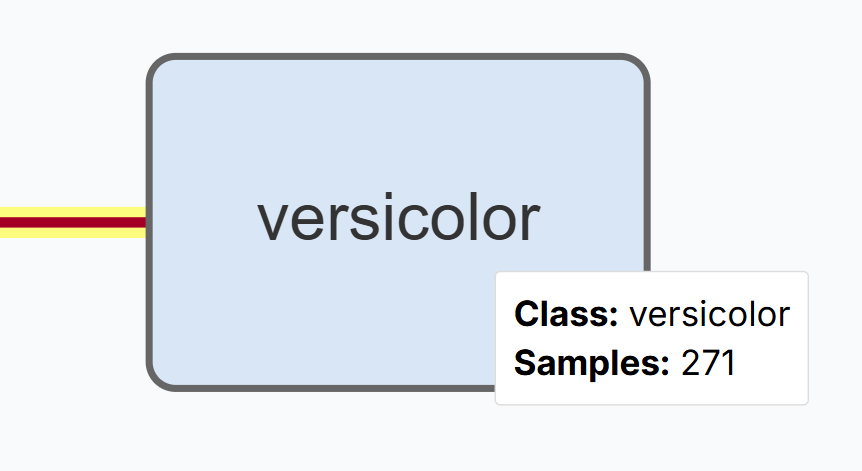
\includegraphics[width=\linewidth]{images/spawnDecisionTreeFinalTooltipLeaf.png}
            \caption{Tooltip on the Rule Centered visualization for a leaf node}
            \label{fig:spawnDecisionTreeFinalTooltipLeaf}
        \end{subfigure}
    \end{subfigure}
    
    \caption{Rule Centered visualization and tooltips.}
\end{figure}

The Rule Centered visualization, shown in Figure \ref{fig:spawnDecisionTreeFinal}, implements a novel \textbf{spawn-based positioning algorithm} that optimizes space utilization while providing enhanced focus on explanation paths. This visualization addresses the challenge of presenting complex tree structures while maintaining clear focus on the instance-specific explanation trajectory.
% 
% \textbf{Spawn-Based Layout Algorithm}: 
The core innovation lies in the \textbf{adaptive spacing mechanism} that adjusts positioning based on subtree complexity. Rather than using uniform spacing between tree levels, the spawn algorithm calculates spacing dynamically based on the size and complexity of subtrees at each level. This approach ensures that complex tree regions receive adequate space while compact regions maintain efficient layouts.

The algorithm specifically analyzes the \textbf{size of subtrees not involved in the explained instance path} and adjusts spacing between path nodes accordingly. When a path node has large subtrees branching off, the horizontal spacing to the next path node increases proportionally, preventing overlap and maintaining visual clarity.
% 
% \textbf{Path-Centric Design Philosophy}: 
The Rule Centered visualization prioritizes the \textbf{explained instance path} through enhanced visual treatment and positioning optimization. Path nodes receive \textbf{rectangular representation} with distinctive styling including thicker borders and brighter colors, while non-path nodes maintain \textbf{circular representation} to visually distinguish between explanation-relevant and contextual information.

% \textbf{Tooltip Information}: 
The Rule Centered visualization provides contextual details consistent with the other tree visualizations. Split node tooltips, shown in Figure \ref{fig:spawnDecisionTreeFinalTooltipSplit}, display feature names, threshold values, impurity measures, sample counts, and class distributions. Leaf node tooltips, shown in Figure \ref{fig:spawnDecisionTreeFinalTooltipLeaf}, present predicted class and sample counts, maintaining the established information architecture across all tree visualizations.

\begin{figure}
    \centering
    \begin{subfigure}[c]{0.48\textwidth}
        \centering
        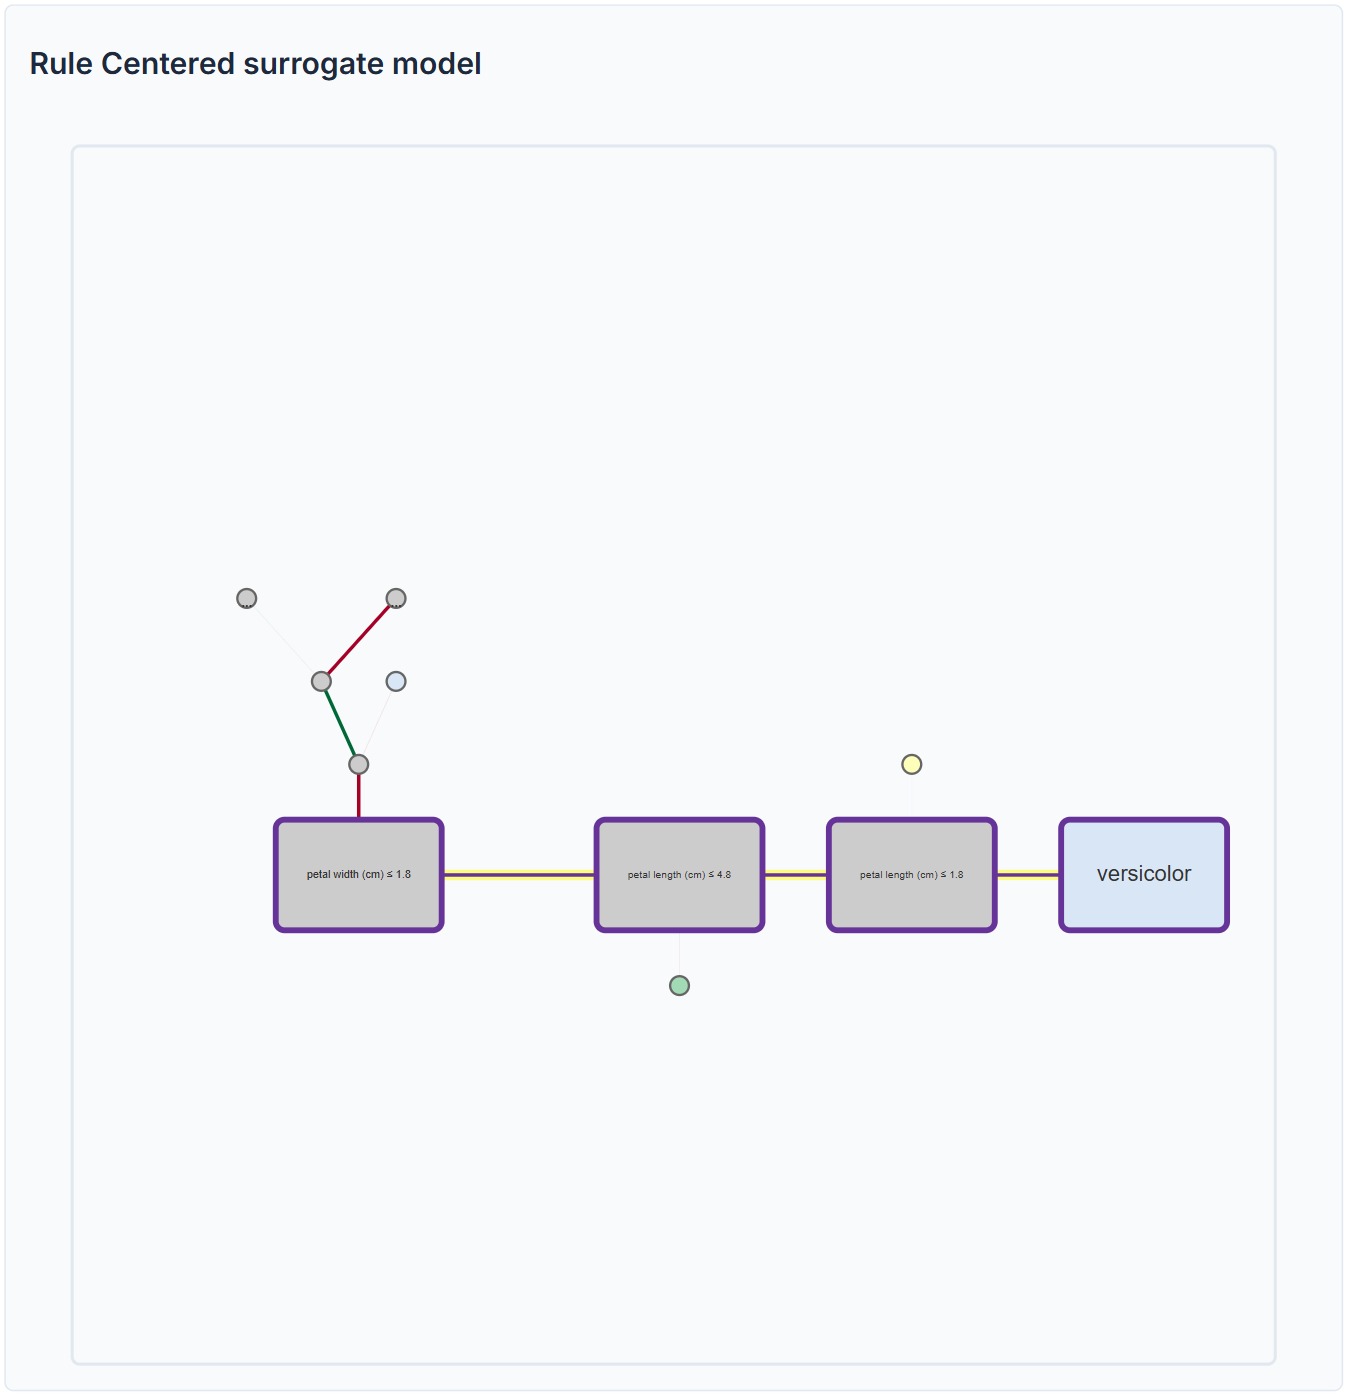
\includegraphics[width=\linewidth]{images/spawnDecisionTreeFinalLeafInteraction.png}
        \caption{Click on leaf node interaction.}
        \label{fig:spawnDecisionTreeFinalLeafClick}
    \end{subfigure}
    \vspace{0.3cm}
    \begin{subfigure}[c]{0.48\linewidth}
        \centering
        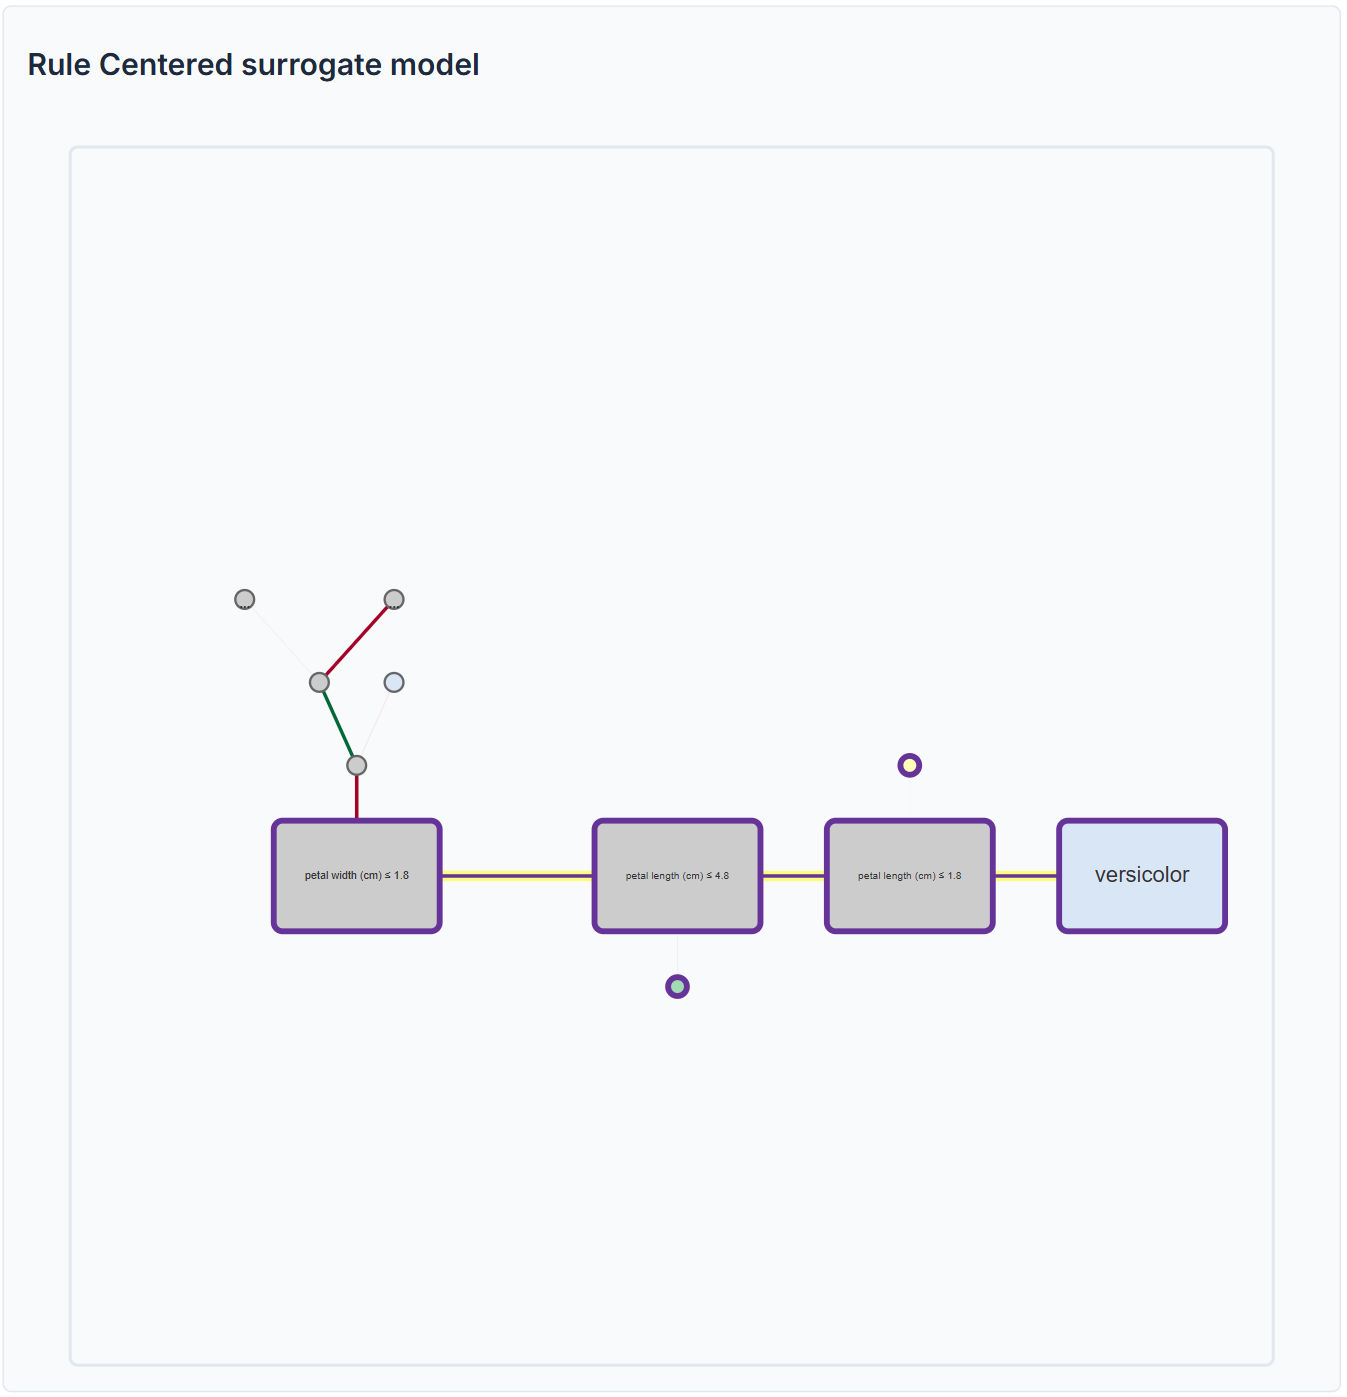
\includegraphics[width=\linewidth]{images/spawnDecisionTreeFinalSplitInteraction.png}
        \caption{Click on split node interaction.}
        \label{fig:spawnDecisionTreeFinalSplitClick}
    \end{subfigure}
    \caption{Rule Centered visualization click interactions.}
\end{figure}

% \textbf{Collapsible Subtree Functionality}: 
A key innovation in the Rule Centered visualization is the implementation of \textbf{interactive subtree collapse/expand functionality}, illustrated in Figure \ref{fig:spawnSubtreeInteractions}. Subtrees not involved in the explained instance path can be collapsed to reduce visual complexity, allowing users to focus on explanation-relevant information while maintaining the option to explore alternative decision paths when needed.

\begin{figure}[ht!]
    \centering
    \begin{subfigure}[c]{0.28\textwidth}
        \centering
        \begin{subfigure}[c]{\linewidth}
            \centering
            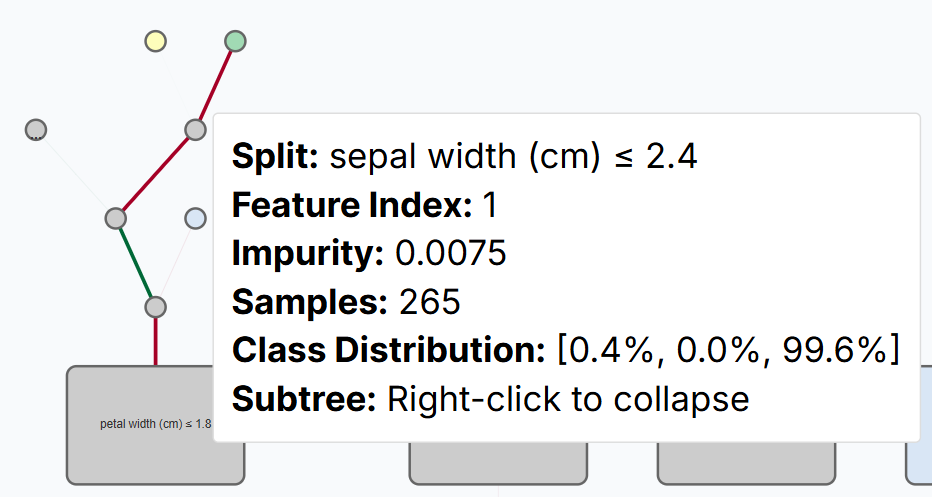
\includegraphics[width=\linewidth]{images/spawnDecisionTreeExpandedHover.png}
            \caption{Hover interaction on an expanded subtree node}
            \label{fig:spawnExpandedHover}
        \end{subfigure}
        \vspace{0.3cm}
        
        \begin{subfigure}[c]{\linewidth}
            \centering
            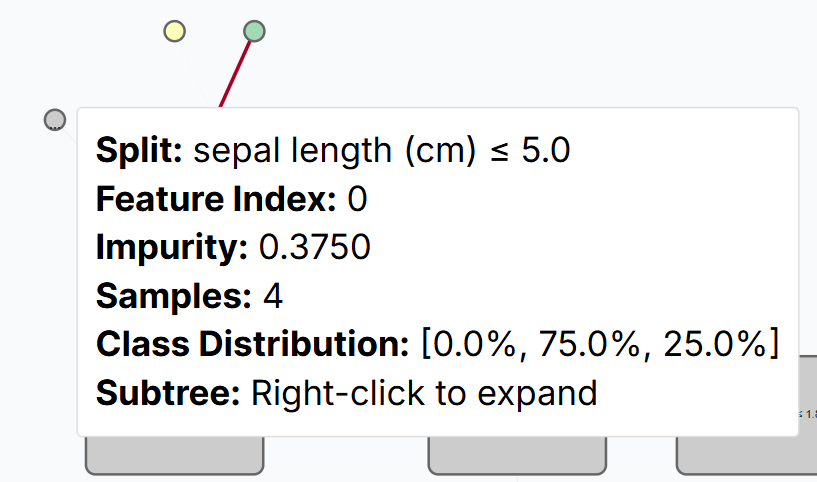
\includegraphics[width=\linewidth]{images/spawnDecisionTreeCollapsedHover.png}
            \caption{Hover interaction on a collapsed subtree node}
            \label{fig:spawnCollapsedHover}
        \end{subfigure}
    \end{subfigure}%
    \hfill
    \begin{subfigure}[c]{0.68\textwidth}
        \centering
        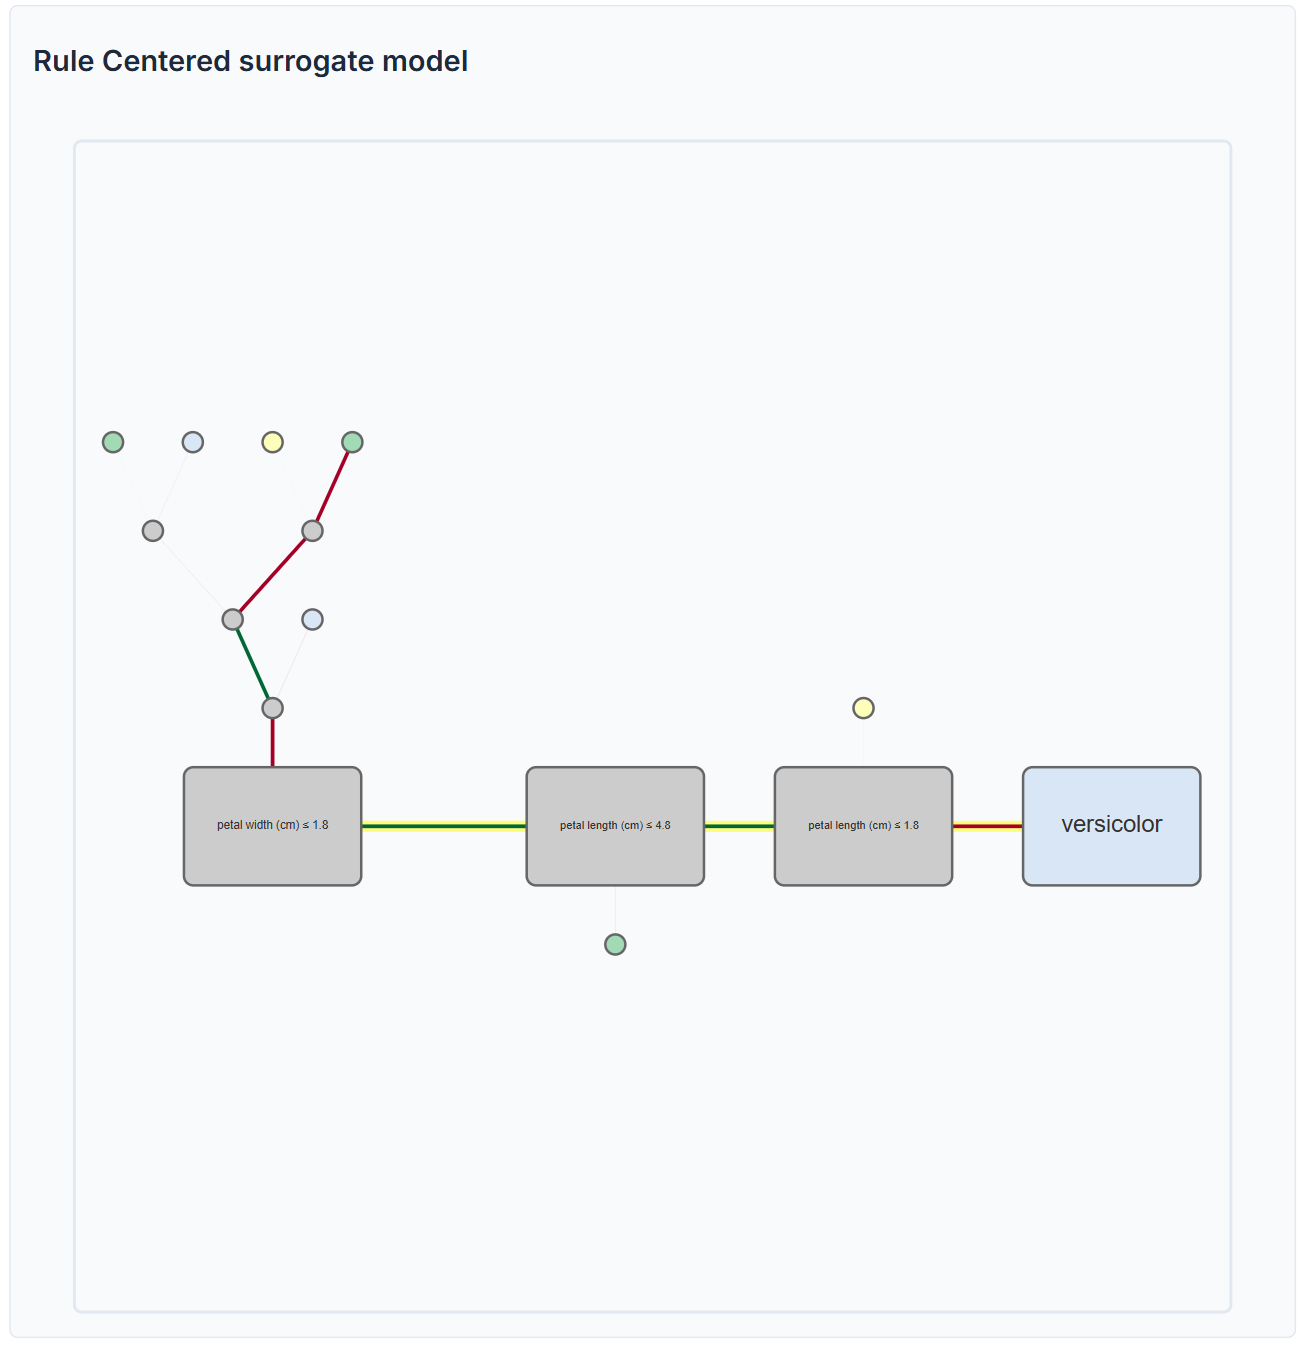
\includegraphics[width=\linewidth]{images/spawnDecisionTreeExpandedSubtree.png}
        \caption{Fully expanded subtree visualization showing additional decision paths}
        \label{fig:spawnExpandedSubtree}
    \end{subfigure}
    
    \caption{Rule Centered visualization subtree collapse/expand interactions and states.}
    \label{fig:spawnSubtreeInteractions}
\end{figure}

Collapsed subtrees are represented by \textbf{simplified placeholder nodes}, shown in Figure \ref{fig:spawnCollapsedHover}, which appear as circles with special visual marking to indicate hidden structure. When users hover over these placeholder nodes, the system provides the \textbf{information} about the collapsed subtree.

Right-click \textbf{context menu interactions} provide intuitive access to subtree expansion controls. When users right-click on a collapsed subtree placeholder node, a context menu appears with options to "Expand Subtree", enabling progressive disclosure of tree complexity. Figure \ref{fig:spawnExpandedSubtree} demonstrates the result of subtree expansion, revealing the complete decision structure that was previously hidden. Expanded subtrees, as shown in Figure \ref{fig:spawnExpandedHover}, can similarly be collapsed through right-click interactions, providing bidirectional control over information density. This interaction pattern supports \textbf{exploratory analysis workflows} where users can progressively reveal complexity as needed rather than confronting the full tree structure immediately.
% 
% \textbf{Adaptive Visual Hierarchy}: 
The spawn tree employs \textbf{visual hierarchy differentiation} to guide user attention effectively. Explained instance path nodes receive enhanced visual treatment through increased size, distinctive rectangular shapes with rounded corners, and prominent borders. The collapsed and expanded states, illustrated in Figure \ref{fig:spawnSubtreeInteractions}, is communicated through smaller circles with special marking, maintain clear visual distinction between explanation-relevant paths and contextual information.
% 
% \textbf{Enhanced Interaction Model}: 
Beyond standard click and hover interactions demonstrated in Figures \ref{fig:spawnDecisionTreeFinalLeafClick} and \ref{fig:spawnDecisionTreeFinalSplitClick}, the spawn tree supports \textbf{contextual interaction modes} that adapt based on node type and state. Path nodes provide detailed explanation information through tooltips showing feature conditions, sample statistics, and impurity measures. Split node clicks trigger the same cross-visualization coordination as other tree types, highlighting corresponding instances in the spatial neighborhood analysis plot. 


\section{Integrated Coordination System}

The final design's greatest strength lies in its \textbf{comprehensive coordination architecture} that seamlessly connects all visualization components through bidirectional interaction mechanisms.

\textbf{Interaction Flow}: When a user clicks a point in the spatial neighborhood analysis plot, as shown in Figure \ref{fig:finalTotalScatterPointClick}, the coordinator identifies the corresponding feature vector, traces the decision path through the rendered tree structure, and propagates highlighting to it. Conversely, when a user clicks a tree node, as shown in Figure \ref{fig:finalTotalTreeLeafClick} the coordinator identifies all synthetic neighborhood instances that satisfy the node's conditions and highlights the corresponding points in the spatial neighborhood analysis plot.

\begin{figure}[ht]
  \centering
  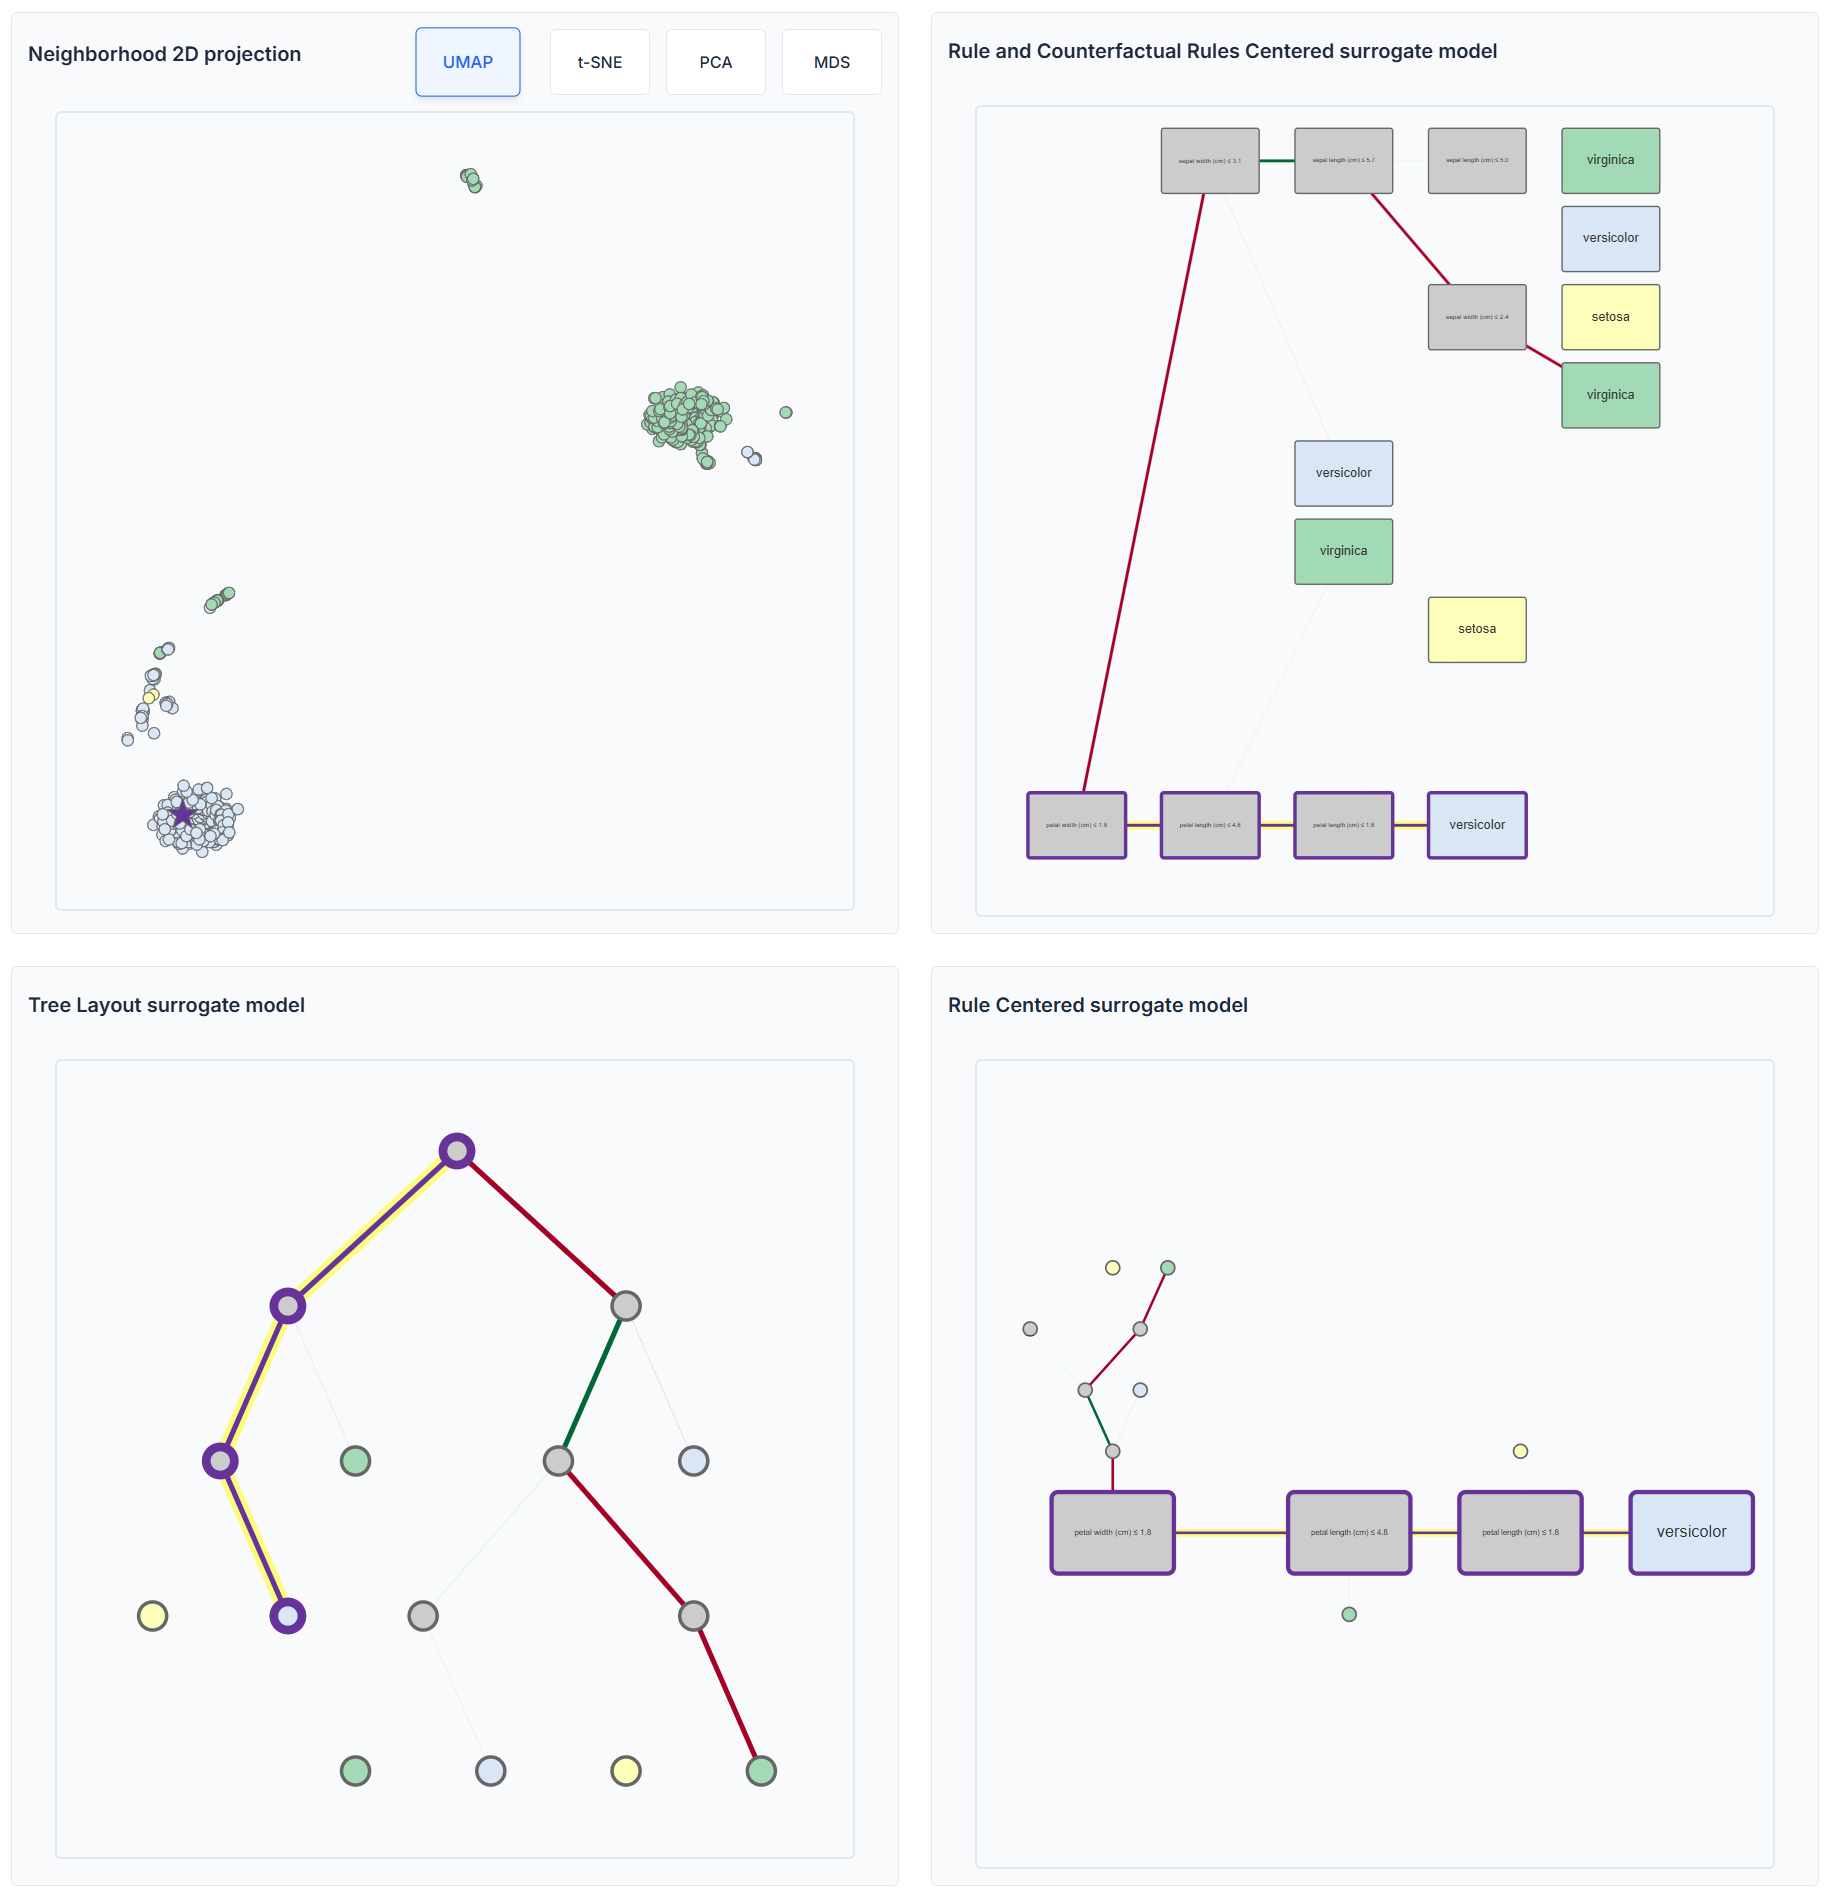
\includegraphics[width=0.7\textwidth]{images/FullInterfaceFinalLeadInteractionScatter.png}
  \caption{Click on spatial neighborhood analysis plot point interaction.}
  \label{fig:finalTotalScatterPointClick}
\end{figure}

\begin{figure}[ht]
  \centering
  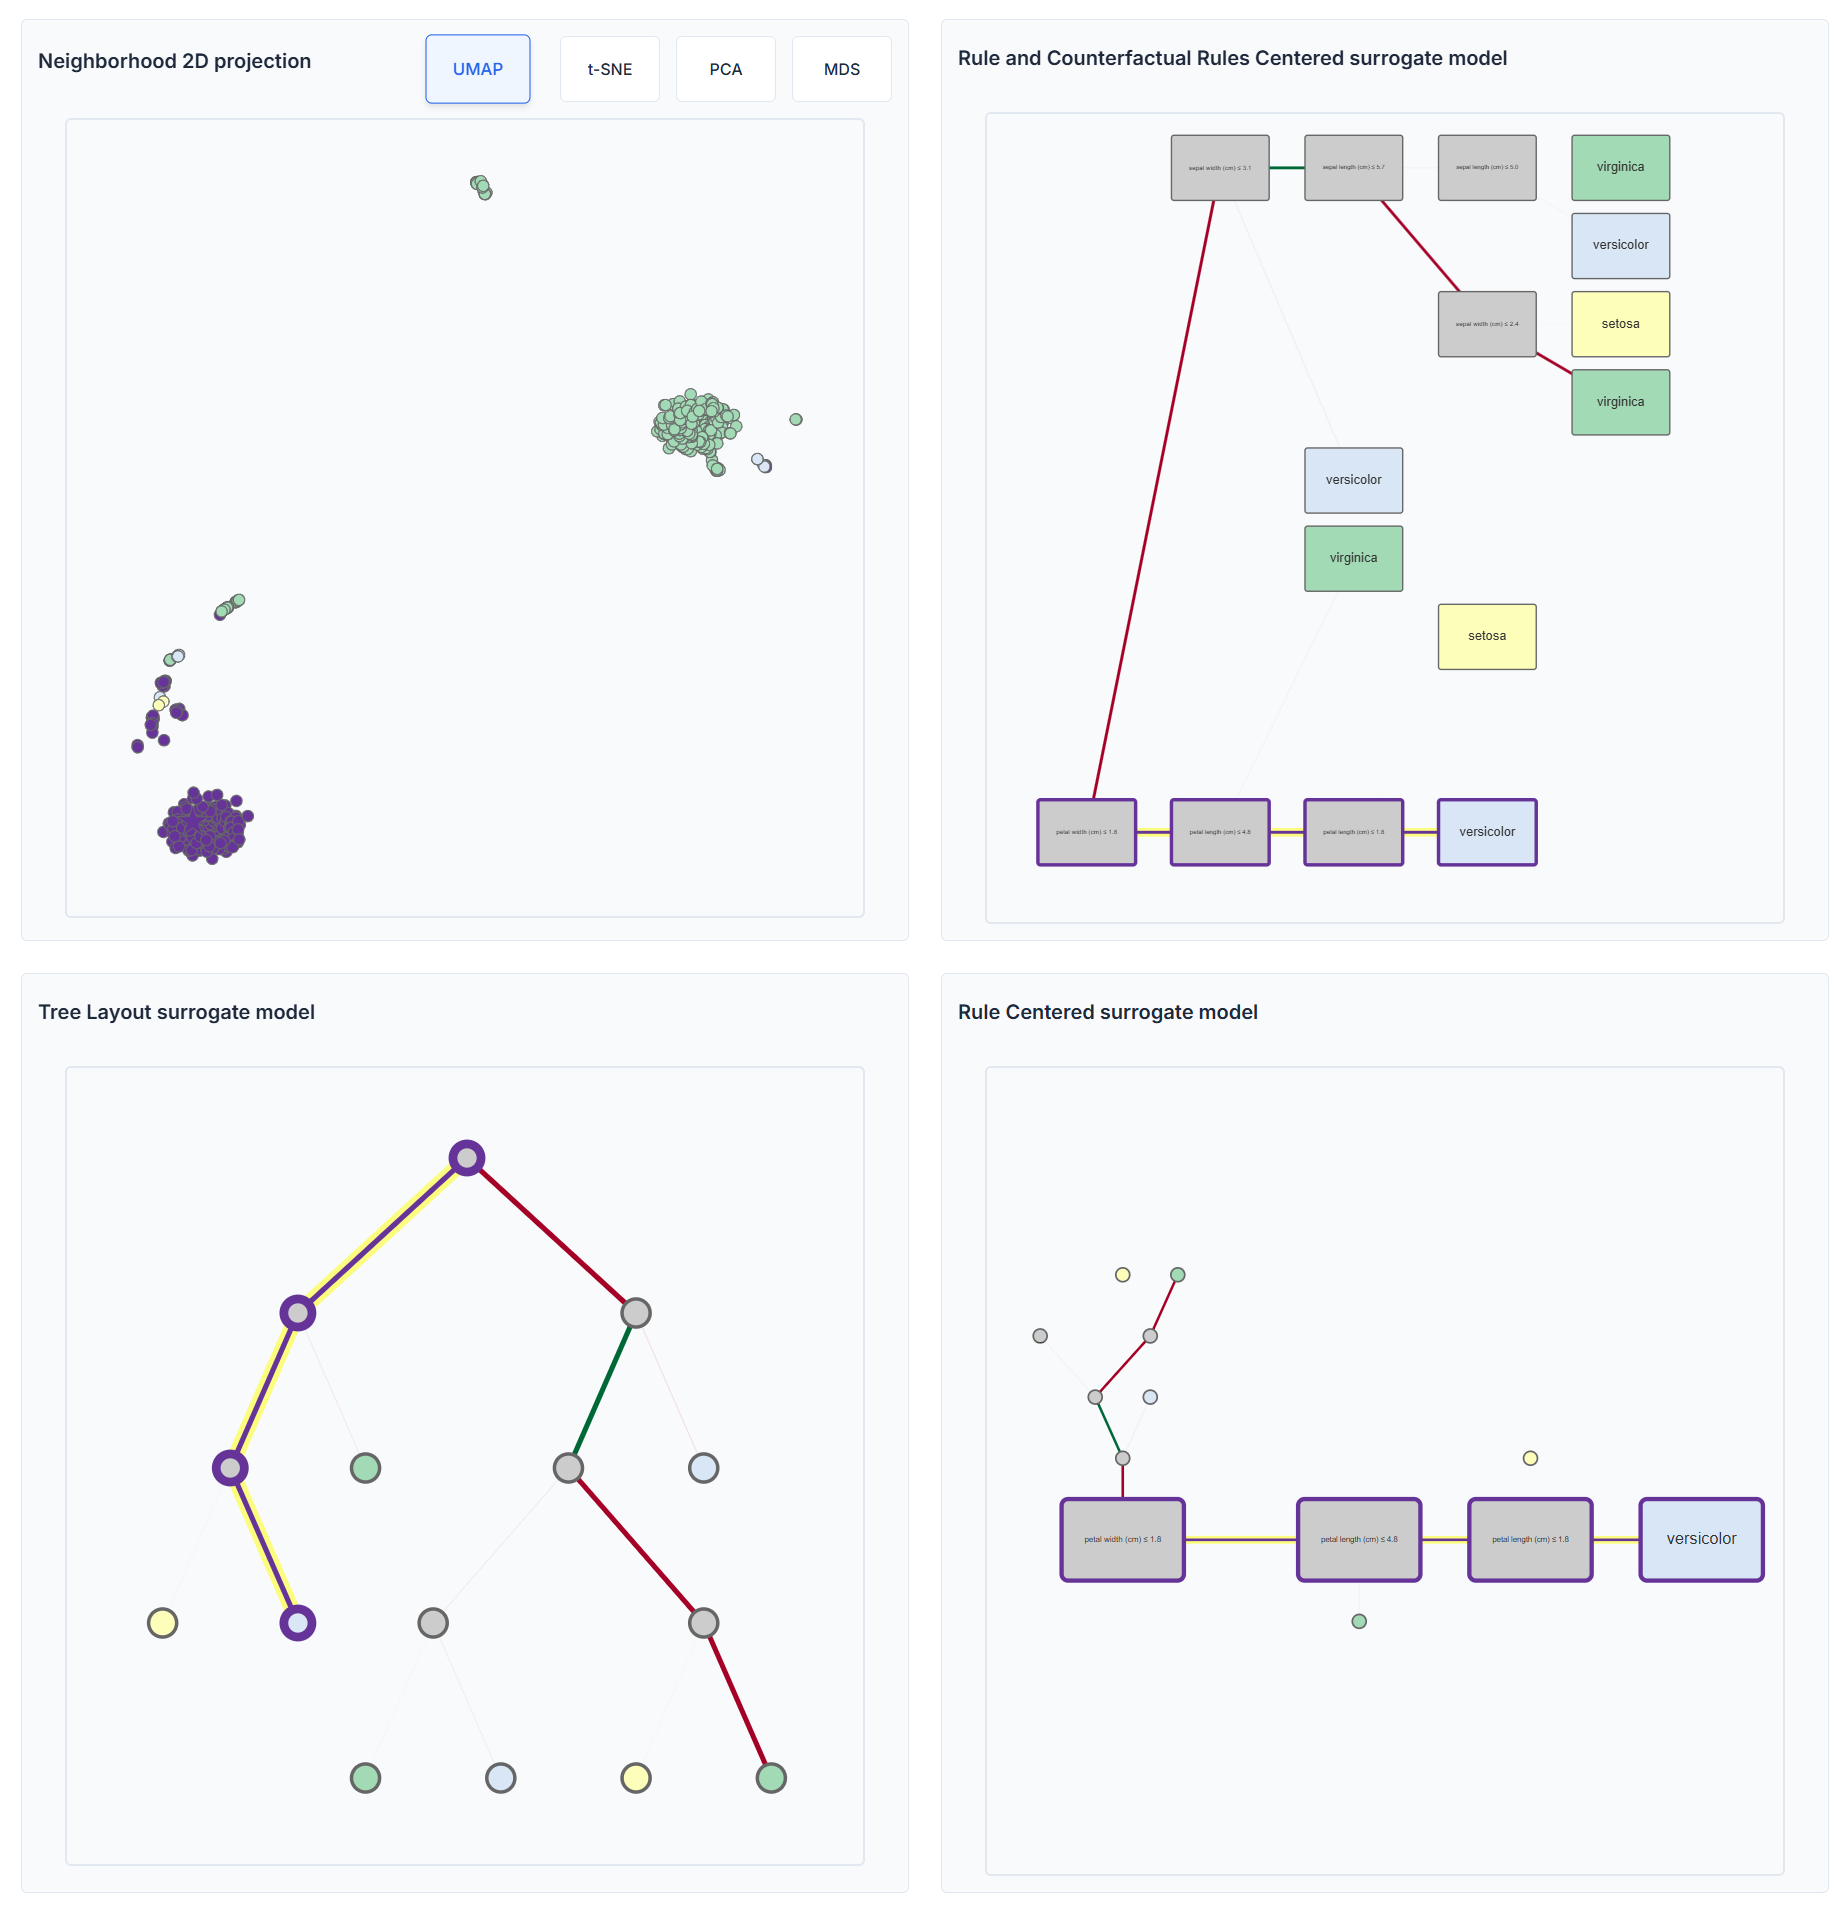
\includegraphics[width=0.7\textwidth]{images/FullInterfaceFinalLeadInteraction.png}
  \caption{Click on decision tree plot interaction.}
  \label{fig:finalTotalTreeLeafClick}
\end{figure}

\textbf{Color Scheme Consistency}: All visualizations employ a unified color scheme, either from the treeviz library \cite{parr2019dtreeviz}, shown in Table \ref{tab:colorBlindPalette}, or, when the number of the dataset classes is higer than 10, the mean points of each class of the dataset are projected in the CIELAB color space with L*=70, ensuring perceptual uniformity across different numbers of target classes. This approach addresses the challenge of maintaining distinguishable colors for datasets with varying numbers of classes (from 2 to 10+) while ensuring consistent visual experience across all visualization components and, up until 10 classes, color-blindness friendliness. 


\begin{table}[!ht]
    \centering
    \caption{Color blind friendly color palettes.}
    \label{tab:colorBlindPalette}
    \resizebox{\textwidth}{!}{%
    \renewcommand{\arraystretch}{2.0} % adjust cell height
    \setlength{\tabcolsep}{4pt}       % horizontal padding
    \small % adjust overall table size if needed
    \begin{tabular}{
        |>{\centering\arraybackslash}m{1.8cm}
        |>{\centering\arraybackslash}m{1.8cm}
        |>{\centering\arraybackslash}m{1.8cm}
        |>{\centering\arraybackslash}m{1.8cm}
        |>{\centering\arraybackslash}m{1.8cm}
        |>{\centering\arraybackslash}m{1.8cm}
        |>{\centering\arraybackslash}m{1.8cm}
        |>{\centering\arraybackslash}m{1.8cm}
        |>{\centering\arraybackslash}m{1.8cm}
        |>{\centering\arraybackslash}m{1.8cm}
        |>{\centering\arraybackslash}m{1.8cm}|
    }
        \hline
        \textbf{Number of Classes} & \textbf{Color 1} & \textbf{Color 2} & \textbf{Color 3} & \textbf{Color 4} & \textbf{Color 5} & \textbf{Color 6} & \textbf{Color 7} & \textbf{Color 8} & \textbf{Color 9} & \textbf{Color 10} \\
        \hline
        2 & \cellcolor[HTML]{FEFEBB}\tiny \#FEFEBB & \cellcolor[HTML]{a1dab4}\tiny \#a1dab4 & & & & & & & & \\
        \hline
        3 & \cellcolor[HTML]{FEFEBB}\tiny \#FEFEBB & \cellcolor[HTML]{D9E6F5}\tiny \#D9E6F5 & \cellcolor[HTML]{a1dab4}\tiny \#a1dab4 & & & & & & & \\
        \hline
        4 & \cellcolor[HTML]{FEFEBB}\tiny \#FEFEBB & \cellcolor[HTML]{D9E6F5}\tiny \#D9E6F5 & \cellcolor[HTML]{a1dab4}\tiny \#a1dab4 & \cellcolor[HTML]{fee090}\tiny \#fee090 & & & & & & \\
        \hline
        5 & \cellcolor[HTML]{FEFEBB}\tiny \#FEFEBB & \cellcolor[HTML]{D9E6F5}\tiny \#D9E6F5 & \cellcolor[HTML]{a1dab4}\tiny \#a1dab4 & \cellcolor[HTML]{41b6c4}\tiny \#41b6c4 & \cellcolor[HTML]{fee090}\tiny \#fee090 & & & & & \\
        \hline
        6 & \cellcolor[HTML]{FEFEBB}\tiny \#FEFEBB & \cellcolor[HTML]{c7e9b4}\tiny \#c7e9b4 & \cellcolor[HTML]{41b6c4}\tiny \#41b6c4 & \cellcolor[HTML]{2c7fb8}\tiny \#2c7fb8 & \cellcolor[HTML]{fee090}\tiny \#fee090 & \cellcolor[HTML]{f46d43}\tiny \#f46d43 & & & & \\
        \hline
        7 & \cellcolor[HTML]{FEFEBB}\tiny \#FEFEBB & \cellcolor[HTML]{c7e9b4}\tiny \#c7e9b4 & \cellcolor[HTML]{7fcdbb}\tiny \#7fcdbb & \cellcolor[HTML]{41b6c4}\tiny \#41b6c4 & \cellcolor[HTML]{225ea8}\tiny \#225ea8 & \cellcolor[HTML]{fdae61}\tiny \#fdae61 & \cellcolor[HTML]{f46d43}\tiny \#f46d43 & & & \\
        \hline
        8 & \cellcolor[HTML]{FEFEBB}\tiny \#FEFEBB & \cellcolor[HTML]{edf8b1}\tiny \#edf8b1 & \cellcolor[HTML]{c7e9b4}\tiny \#c7e9b4 & \cellcolor[HTML]{7fcdbb}\tiny \#7fcdbb & \cellcolor[HTML]{1d91c0}\tiny \#1d91c0 & \cellcolor[HTML]{225ea8}\tiny \#225ea8 & \cellcolor[HTML]{fdae61}\tiny \#fdae61 & \cellcolor[HTML]{f46d43}\tiny \#f46d43 & & \\
        \hline
        9 & \cellcolor[HTML]{FEFEBB}\tiny \#FEFEBB & \cellcolor[HTML]{c7e9b4}\tiny \#c7e9b4 & \cellcolor[HTML]{41b6c4}\tiny \#41b6c4 & \cellcolor[HTML]{74add1}\tiny \#74add1 & \cellcolor[HTML]{4575b4}\tiny \#4575b4 & \cellcolor[HTML]{313695}\tiny \#313695 & \cellcolor[HTML]{fee090}\tiny \#fee090 & \cellcolor[HTML]{fdae61}\tiny \#fdae61 & \cellcolor[HTML]{f46d43}\tiny \#f46d43 & \\
        \hline
        10 & \cellcolor[HTML]{FEFEBB}\tiny \#FEFEBB & \cellcolor[HTML]{c7e9b4}\tiny \#c7e9b4 & \cellcolor[HTML]{41b6c4}\tiny \#41b6c4 & \cellcolor[HTML]{74add1}\tiny \#74add1 & \cellcolor[HTML]{4575b4}\tiny \#4575b4 & \cellcolor[HTML]{313695}\tiny \#313695 & \cellcolor[HTML]{fee090}\tiny \#fee090 & \cellcolor[HTML]{fdae61}\tiny \#fdae61 & \cellcolor[HTML]{f46d43}\tiny \#f46d43 & \cellcolor[HTML]{d73027}\tiny \#d73027 \\
        \hline
    \end{tabular}%
    }
\end{table}

The final design successfully integrates the spatial and symbolic representation paradigms through coordinated multiple views, providing users with comprehensive tools to confirm, explore, and understand the generated explanations. The configuration interface enables flexible control over the explanation generation process, while the multi-tree approach accommodates diverse cognitive preferences, and the spatial neighborhood analysis plot provides essential spatial context for understanding neighborhood quality and decision boundary characteristics.

